\documentclass[oneside,a4paper]{book}

\usepackage[pdftex]{graphicx}
\usepackage{amsmath}
\usepackage{amssymb}
\usepackage{textcomp}
\usepackage[utf8]{inputenc}
\usepackage[polish]{babel}
\usepackage[T1]{fontenc}
\usepackage{array}
\usepackage{tabularx}
\usepackage{enumitem}
\usepackage[justification=centering]{caption}

\raggedbottom

% pakiet stosowany do url'i w bibliografii, zamienia odnośniki na ładnie sformatowane
\usepackage{url}
% pakiety służące do numerowania i tworzenia algorytmów
\usepackage{algorithmic}
\usepackage{algorithm}
% redefinicja etykiety nagłówkowej listy algorytmów, domyślna jest po angielsku
\renewcommand{\listalgorithmname}{Spis algorytmów}

% pakiet do wyliczania skali, przydatny przy dużych obrazkach
\usepackage{pgf}
% pakiet służący do automatycznego sortowania odnośników do bibliografii
\usepackage[sort]{natbib}
% tworzenie listingów
\usepackage{listings}
% tworzenie figur wewnątrz figur
\usepackage{subfig}
% do automatycznego skracania nazw rozdziałów i podrozdziałów używanych w nagłówkach strony by mieściły się w jednej linii
\usepackage[fit]{truncate}
% fancyhdr - ładne nagłówki, definicja wyglądu nagłówka, numery stron będą umieszczane w nagłówku po odpowiedniej stronie
\usepackage{fancyhdr}
\pagestyle{fancy}
\renewcommand{\chaptermark}[1]{\markboth{#1}{}}
\renewcommand{\sectionmark}[1]{\markright{\thesection\ #1}}
\fancyhf{}
\fancyhead[LE,RO]{\bfseries\thepage}
% tutaj ograniczamy szerokość pola w nagłówku zawierającego nazwę rozdziału/podrozdziału do 95% szerokości strony
% redefinicja sposobu prezentacji nazw domyślnie wypisywanych wielkimi literami (np. domyślnie w nagłówku Spis treści będzie miał postać SPIS TREŚCI)
% Uwaga! to może popsuć wielkie litery w ogóle! Jak coś nie działa należy usunąć \nouppercase{} z poniższych definicji
\fancyhead[LO]{\nouppercase{\bfseries{\truncate{.95\headwidth}{\rightmark}}}}
\fancyhead[RE]{\nouppercase{\bfseries{\truncate{.95\headwidth}{\leftmark}}}}
\renewcommand{\headrulewidth}{0.5pt}
\renewcommand{\footrulewidth}{0pt}

% definicja typu prostego wymagana przez pierwsze strony rozdziałów itp.
% powyższe reguły niestety tych stron nie dotyczą, gdyż Latex automatycznie przełącza je pomiędzy fancy a plain
% w tym wypadku eliminujemy nagłówki i stopki na stronach początkowych
\fancypagestyle{plain}{%
 \fancyhead{}
 \fancyfoot{}
 \renewcommand{\headrulewidth}{0pt}
 \renewcommand{\footrulewidth}{0pt}
}

%\parskip 0.5in

% makro umożliwiające otaczanie symboli okręgami
\usepackage{tikz}
% brak justowania tekstu (bazą okręgu będzie linia tekstu)
\newcommand*\mycirc[1]{%
  \begin{tikzpicture}
    \node[draw,circle,inner sep=1pt] {#1};
  \end{tikzpicture}}

% pionowe justowanie tekstu, środek okręgu pokrywa się ze środkiem tekstu
\newcommand*\mycircalign[1]{%
  \begin{tikzpicture}[baseline=(C.base)]
    \node[draw,circle,inner sep=1pt](C) {#1};
  \end{tikzpicture}}

% zmiana nazwy twierdzeń i lematów
\newtheorem{theorem}{Twierdzenie}[section]
\newtheorem{lemma}[theorem]{Lemat}

% tworzenie definicji dowodu
\newenvironment{proof}[1][Dowód]{\begin{trivlist}
\item[\hskip \labelsep {\bfseries #1}]}{\end{trivlist}}
% \newenvironment{definition}[1][Definicja]{\begin{trivlist}
% \item[\hskip \labelsep {\bfseries #1}]}{\end{trivlist}}
% \newenvironment{example}[1][Przykład]{\begin{trivlist}
% \item[\hskip \labelsep {\bfseries #1}]}{\end{trivlist}}
% \newenvironment{remark}[1][Uwaga]{\begin{trivlist}
% \item[\hskip \labelsep {\bfseries #1}]}{\end{trivlist}}

% definicja czarnego prostokąta zwyczajowo dodawanego na koniec dowodu
\newcommand{\qed}{\nobreak \ifvmode \relax \else
      \ifdim\lastskip<1.5em \hskip-\lastskip
      \hskip1.5em plus0em minus0.5em \fi \nobreak
      \vrule height0.75em width0.5em depth0.25em\fi}

% poniższymi instrukcjami można sterować co ma być numerowane a co nie i co ma być wyświetlane w spisie treści
% \setcounter{secnumdepth}{3}
% \setcounter{tocdepth}{5}

% definicja czcionki mniejszej niż tiny (domyślnie takiej małej nie ma)
\usepackage{lmodern}
\makeatletter
  \newcommand\tinyv{\@setfontsize\tinyv{4pt}{6}}
\makeatother

% definicja jeszcze mniejszej czcionki
\usepackage{lmodern}
\makeatletter
  \newcommand\tinyvv{\@setfontsize\tinyvv{3.5pt}{6}}
\makeatother

% pakiet do obsługi wielostronicowych tabel
\usepackage{longtable}
\setlength{\LTcapwidth}{\textwidth}

\usepackage[section] {placeins}
\usepackage{multirow}
\usepackage{slantsc}

% interlinia
\usepackage{setspace}

% korekta marginesów - domyślnie latex ma jakieś kosmiczne
\usepackage{anysize}
\marginsize{3.5cm}{2.5cm}{2.5cm}{2.5cm}
% po zmianie marginesów konieczne jest wymuszenie przeliczenia nagłówków
\fancyhfoffset[E,O]{0pt}

\usepackage{titlesec}
\titlespacing*{\chapter}{0pt}{-50pt}{20pt}
\titleformat{\chapter}[display]{\normalfont\huge\bfseries}{\chaptertitlename\ \thechapter}{20pt}{\huge}

\setlength{\LTleft}{0pt}
\setlist[itemize]{nolistsep}
\setlist[enumerate]{nolistsep}
\begin{document}

\begin{titlepage}
\begin{center}

% Nagłówek

\includegraphics[width=0.3\textwidth]{img/put_logo.png}\\[0.1in]
\Large{Instytut Informatyki}\\
\normalsize
Wydział Informatyki\\
Politechnika Poznańska\\
ul. Piotrowo 2, Poznań \\[2cm]

\Large{PRACA DYPLOMOWA MAGISTERSKA}\\[1cm]

% Title
\Large \textbf {System wspomagający jednoczesne stosowanie wielu wytycznych klinicznych dla jednego pacjenta}\\[2cm]
% Submitted by
\begin{table}[h]
\centering
\begin{tabular}{lr}\hline \\ 
Dariusz Radka & 100383 \\ \\ \hline 
\end{tabular}
\end{table}

\vspace{1cm}

\normalsize Promotor \\
\begin{table}[h]
\centering
\begin{tabular}{c}\hline \\
dr hab. inż. Szymon Wilk \\ \\ \hline 
\end{tabular}
\end{table}

\vspace{2cm}
Poznań, 2015

\vfill

\end{center}

\end{titlepage}

% sekcja wstępna książki, numerowana rzymskimi
\frontmatter
% generacja strony tytułowej załączonej wcześniej
% \maketitle
% spis treści
\tableofcontents

% dodatkowa strona z podaniem źródła finansowania itp.
% wstawienie pustego symbolu
\null
% i wypełnienie nim całej dostępnej strony
\vfill
% a na jej dole dodajemy właściwy tekst
% w tym przypadku z wyrównaniem do prawej strony

% właściwa część książki, numerowana arabskimi od 1
\mainmatter
\def\arraystretch{1.5}

\chapter{Wstęp}
\section{Wprowadzenie}

\begin{spacing}{1.5}

Szybki rozwój medycyny (np. pojawianie się nowych leków, testów i procedur), rosnąca lawinowo ilość gromadzonych danych klinicznych, a także pojawianie się coraz większej liczby złożonych przypadków (co jest spowodowane m.in. starzeniem się społeczeństw) powoduje, że coraz bardziej istotne staje się wspomaganie lekarzy podczas podejmowania decyzji diagnostycznych i terapeutycznych. W tym celu tworzy się systemy wspomagania decyzji klinicznych (SWDK), przez które rozumie się wszelkie systemy komputerowe pomagające personelowi medycznemu podejmować decyzje\cite{Musen06}. Wśród SWD wyróżnia się: systemy do zarządzania informacją i wiedzą, systemy do zwracania uwagi, przypominania i alarmowania oraz systemy do opracowywania zaleceń.

DO SWDK z pierwszej grupy zalicza się wszelkie systemy służące do zbierania, przechowywania i udostępniania danych pacjentów. Przykładem takiego systemu jest Eskulap tworzony przez pracowników Politechniki Poznańskiej. Eskulap jest skierowany dla różnych placówek medycznych, m. in. szpitali, przychodni oraz aptek. Korzysta z niego wiele placówek na terenie całej Polski. Eskulap składa się z kilkudziesięciu modułów, m.in. eRejestracja, Apteka, Laboratorium, Elektroniczna Dokumentacja Medyczna. Do SWDK z drugiej grupy należą systemy wbudowywane w aparaturę pomiarową (np. monitorującą funkcje życiowe) lub laboratoryjną. Dzięki czemu na bieżąco można informować personel kliniczny o niewłaściwych (np. wykraczających poza normy) wartościach obserwowanych lub testowanych parametrów. Wreszcie do trzeciej grupy SWDK należą systemy, które dla konkretnego pacjenta przygotowują sugestie diagnostyczne i terapeutyczne, korzystając przy tym z szeroko rozumianych modeli decyzyjnych, które stosowane są do dostępnych danych pacjenta. 

Znanym przykładem diagnostycznego SWDK jest system Isabel \cite{Isabel}, który wykorzystuje model decyzyjny w formie odpowiednio poindeksowanych publikacji medycznych. Objawy i cechy charakterystyczne pacjenta są wprowadzane do systemu w formie tekstowej (mogą być także pobierane z elektronicznej karty pacjenta). System dopasowuje je do dostępnych publikacji i na podstawie tego dopasowania tworzy listę możliwych diagnoz dla pacjenta. Dodatkowo, istnieje możliwość przeglądana fragmentów publikacji, które związane są z poszczególnymi diagnozami. 

W praktyce większą popularność zyskują wytyczne postępowania klinicznego (ang. \textit{clinical practice guidelines}, CPG), które pozwalają opisać postępowanie dla pacjenta chorującego na określoną chorobę. Takie wytyczne są coraz częściej formalizowane oraz osadzane w SWDK w celu planowania i nadzorowania wykonywania terapii. Niestety, większość wytycznych jest opracowywana przy założeniu, że pacjent cierpi tylko na jedną przypadłość, co jest bardzo dużym ograniczeniem praktycznym. Z uwagi na proces starzenia się społeczeństw wzrasta liczba pacjentów, którzy cierpią jednocześnie na wiele schorzeń. W takich sytuacjach bezkrytyczne jednoczesne stosowanie wielu wytycznych może przynieść efekt odwrotny do zamierzonego, tzn. może pogorszyć jakość oferowanej opieki \cite{Boyd05}. Dlatego też niezwykle istotne jest szybkie wykrywanie możliwych konfliktów (niekorzystnych interakcji) pomiędzy wytycznymi i wprowadzenie takich zmian w wytycznych, aby uniknąć lub osłabić te konflikty. Wprowadzane zmiany mogą polegać na wprowadzeniu zamienników dla konfliktowych leków, przepisaniu dodatkowych leków, zmianie dawek leków lub też rezygnacji z części leków.

O znaczeniu problemu wykrywania i usuwania konfliktów między wytycznymi świadczy to, iż jest on jednym z „wielkich wyzwań” dla wspomagania decyzji klinicznych \cite{Sittig08}. Niniejsza praca jest próbą zmierzenia się z tym wyzwaniem poprzez opracowanie SWDK  wspomagającego jednoczesne stosowanie wielu wytycznych dla jednego pacjenta. 


\section{Cel i zakres pracy}

Cele główne pracy magisterskiej są następujące:
\begin{enumerate}
\item rozszerzenie podejścia do wykrywania i usuwania konfliktów wykorzystującego programowanie logiczne z ograniczeniami i opisanego w \cite{SzWilk2},
\item implementacja rozszerzonego podejścia w formie samodzielnego SWDK.
\end{enumerate}
Pierwszy z celów głównych wiąże się z następującymi celami szczegółowymi:
\begin{enumerate}
\item umożliwieniem stosowania więcej niż dwóch wytycznych, 
\item dopuszczeniem stosowania wielu zmian w wytycznych (wielu operacji modyfikujących wytyczne), 
\item uwzględnieniem stosowania dawek zarówno przy wykrywaniu konfliktów, jak i wprowadzania zmian w wytycznych.
\end{enumerate}
Drugi z celów głównych jest zdekomponowany na następujące cele szczegółowe:
\begin{enumerate}
\item opracowanie reprezentacji dla wytycznych, opisu konfliktów i wprowadzanych zmian,
\item uwzględnienie dodatkowych danych pacjenta, które nie występują w wytycznych, a które należy uwzględnić podczas wykrywania konfliktów,
\item stworzenie SWD pozwalającego na krokowe wykonywanie wytycznych, wyszukiwanie konfliktów oraz wprowadzanie zmian w wytycznych. System ten ma zostać zaimplementowany w języku Java oraz ma korzystać z dodatkowych bibliotek dostępnych na licencji \textit{open source}.
\end{enumerate}


\section{Struktura pracy}

W rozdziale 2 krótko omówiono wytyczne postępowania klinicznego oraz ich rolę w medycynie. W tym rozdziale zaprezentowano także podejścia do wykrywania i usuwania interakcji w wytycznych postępowania klinicznego. Rozdział 3 opisuje paradygmat programowania logicznego z ograniczeniami. Opisano w tym rozdziale podstawowe właściwości podejścia, a także zamieszczono przykład ilustrujący jego wykorzystanie. W rozdziale 4 zaprezentowano narzędzia i biblioteki użyte podczas wykonywania pracy magisterskiej. Rozdział 5 opisuje główną część pracy, czyli rozszerzenie podejścia do wykrywania i usuwania konfliktów oraz implementację systemu. W tym rozdziale przedstawiono poszczególne części systemu. Rozdział 6 prezentuje działanie systemu na wybranych scenariuszach klinicznych. Rozdział 7 stanowi wreszcie podsumowanie pracy. 


\chapter{Przegląd literatury}
\section{Wytyczne postępowania klinicznego}

% SW: Poniższy opis jest mocno zagmatwany i nie do końca wiadomo, jaka jest jego główna myśl przewodnia. Opisując wytyczne powinien Pan uwzględnić nastepujące elementy:
% (1) definicja wytycznych (mniej lub bardziej sformalizowany opis postępowania z pacjentem ze specyficznym problemem) oraz ich cel (standaryzacja opieki, ograniczenie zmienności w postępowaniu),
% (2) sposoby reprezentowania wytycznych (dokumenty tekstowe, reprezetacje formalne, w tym grafowe),
% (3) implementacja wytycznych w formie systemów komputerowych (możliwość personalizacji wytycznych i wykorzystania dostępnych danych pacjenta)
% (4) konflikty/interakcje wynikające ze stosowania wielu wytycznych jako jeden z głównych problemów ograniczających praktyczne wykorzystanie wytycznych oraz jedno z głównych wyzwań dla SWDK 
% W tym rozdziale mógłby zamieścić Pan przykłady różnych reprezentacji wytycznych (np. w formie tekstu oraz w formie grafu)
Wytyczne postępowania klinicznego\cite{Boyd, Latoszek-Berendsen} to dokument, którego zadaniem jest pomoc lekarzom i personelowi medycznemu w podejmowaniu decyzji związanych z określonymi obszarami opieki medycznymi, w szczególności z leczeniem pacjentów z różnych dolegliwości. Kolejnym celem wytycznych jest poprawa jakości opieki medycznej poprzez jej standaryzację i zwiększenie wydajności personelu medycznego. Dzięki temu można obniżyć koszty usług czy zlecanych badań. Wytyczne są tworzone przez ekspertów medycznych. Rozwój wytycznych wysokiej jakości wymaga specjalistycznego zespołu ludzi i wystarczającego budżetu. Wytyczne postępowania klinicznego mogą mieć różną reprezentację. Do przykładowych reprezentacji należą dokumenty tekstowe oraz reprezentacje formalne takie, jak tablice decyzyjne czy formaty grafowe. Implementacja wytycznych w formie systemów komputerowych daje możliwość personalizacji wytycznych, czyli uwzględnia osobistą charakterystykę pacjenta. Komputerowo interpretowane wytyczne, które posiadają dostęp do elektronicznego rekordu pacjenta, są w stanie dostarczyć porady dotyczące konkretnego pacjenta. Niestety, wytyczne dotyczą z reguły jedynie konkretnej dolegliwości. W związku z tym, wytyczne w przypadku pacjentów chorujących na kilka chorób, którymi często są osoby starsze, mogą doprowadzić do niewłaściwego wyboru terapii. Ważnym aspektem w tej kwestii jest znajdowanie konfliktów występujących między wytycznymi i ich odpowiedniego rozwiązania.


%Wytyczne postępowania klinicznego\cite{Boyd, Latoszek-Berendsen} pozwalają polepszyć jakość opieki medycznej. Wytyczne są tworzone przez ekspertów medycznych. Rozwój wytycznych wysokiej jakości wymaga specjalistycznego zespołu ludzi i wystarczającego budżetu. Wytyczne powinny oferować spersonalizowane porady. Komputerowo interpretowane wytyczne, które posiadają dostęp do elektronicznego rekordu pacjenta, są w stanie dostarczyć porady dotyczące konkretnego pacjenta. Wytyczne wpływają pozytywnie na pracę personelu medycznego i zwiększają wydajność. Pacjenci mogą czerpać korzyści z wytycznych, które podsumowują zalety i wady możliwych opcji. Pacjenci mogą się dowiedzieć więcej o wyborach medycznych, które uwzględniają ich osobistą charakterystykę. Cały system medyczny może dzięki wytycznym zwiększyć wydajność, co może obniżyć koszty usług, przepisywanych leków czy zlecanych badań. Wytyczne w przypadku pacjentów chorujących na kilka chorób, którymi często są osoby starsze, mogą doprowadzić do niewłaściwego wyboru terapii. Ważnym aspektem w tej kwestii jest znajdowanie konfliktów występujących między wytycznymi i ich odpowiedniego rozwiązania.

% SW: Proszę się zdecydowac na jeden termin -- interakcje albo konflikty -- i konsekwetnie stosować go w całym tekście. Może warto zdecydować się na termin "konflikt" -- interakcje mogą być również poztywne (jedno działanie korzystnie wzmacnia inne), jednak tymi się nie zajmujemy.
\section{Wykrywanie i usuwanie konfliktów w wytycznych postępowania klinicznego}

% SW: Tutaj powinien też znaleźć sie opis naszego podejścia z pracy JBI (cytowanie podałem wcześniej), ponieważ właśnie je Pan rozszerza.
\subsection{Programowanie logiczne z ograniczeniami}
Wytyczne postępowania klinicznego są w tej technice prezentowane w postaci grafu akcji.\cite{SzWilk2} Graf akcji jest grafem skierowanym, na który składają się trzy typy węzłów. Pierwszy typ to węzeł kontekstu. Jest to węzeł początkowy opisujący określoną chorobę. Kolejnym typem jest węzeł akcji, który opisuje akcję medyczną, którą należy wykonać. Ostatnim typem jest węzeł decyzji, który zawiera pytanie, na które należy odpowiedzieć. Graf akcji jest w tym podejściu transformowany następnie do modelu logicznego. Model ten składa się z wyrażeń logicznych opisujących poszczególne ścieżki w grafie. Akcje, których nie ma na ścieżce   są zapisywane w wyrażeniu w postaci negacji. W tym podejściu stosowane są także tzw. operatory interakcji i rewizji. Operator interakcji reprezentuje niepożądany konflikt (zazwyczaj lek-lek lub lek-choroba), który jest w postaci zdania zbudowanego z elementów wyrażeń logicznych modelu logicznego. Operator rewizji opisuje natomiast zmiany, jakie należy wprowadzić do modeli logicznych, aby konflikt usunąć. Modele logiczne reprezentujące wytyczne są zamieniane na programy CLP, które są automatycznie wykonywane. Uzyskane rozwiązanie wskazuje na ścieżki, jakie należy przejść podczas leczenia pacjenta.


\subsection{Logika pierwszego rzędu}

% SW: grafy akcji stosowane są także w naszym podejściu z CLP jako pośrednia reprezentacja wytycznych, uniezleżniająca nas od specyficznego języka reprezentacji. Również w podejściu z CLP korzystaliśmy z operatorów interakcji (opisujących konflikty) oraz rewizji (naprawiających/usuwających konflikty).
% SW: Podejście wykorzystujące FOL miało podobne cele, jak te realizowane w Pańskiej pracy -- możliwość stosowania wielu wytycznych oraz operatorów oraz uwzględnianie dawek leków. Dodatkowo FOL, dzięki predykatom, oferuje większą czytelność uzyskiwanych rozwiązań. Minusem są bardziej złożone modele reprezentujące wytyczne oraz konieczność stosowania bardziej złożonych narzędzi (m.in. systemów do dowodzenia twierdzeń). Pańska praca ma na celu sprawdzenie, co możemy jeszcze "wycisnąć" z CLP bez konieczności sięgania po FOL.

% SW: W poniższym opisie powinien się Pan skupić na tych elementach pojdeścia, o których wspomniałem powyżej (stosowaniu wielu wytycznych i wykrywania/naprawiania wielku konfliktów). Jak już wspomniałem, wiele elementów zostnie już opisanych przy okazji przedstawienia naszego podejścia z CLP.

Wytyczne postępowania klinicznego są w tym podejściu opisane, podobnie jak w poprzednim podejściu, za pomocą grafu akcji z węzłami kontekstu, decyzji i akcji.\cite{SzWilk} Słownictwo podejścia logiki pierwszego rzędu składa się ze stałych (pisanych dużymi literami), zmiennych (pisanych małymi literami) oraz predykatów. Do predykatów należą:
\begin{itemize}
\item{node(x) – x jest węzłem}
\item{action(x) – x jest węzłem akcji}
\item{decision(x) – x jest węzłem decyzji}
\item{executed(x) – węzeł akcji x jest zastosowany}
\item{value(x, v) – wartość v jest związana z węzłem decyzji x}
\item{dosage(x, n) – węzeł akcji x jest opisany przez dawkę n}
\item{directPrec(x, y) – węzeł x poprzedza bezpośrednio węzeł y}
\item{prec(x, y) – węzeł x poprzedza węzeł y}
\item{disease(d) – d jest chrobą}
\item{diagnosed(d) – pacjent choruje na chorobę d}
\end{itemize}
W tym podejściu także stosowane są operatory interakcji i rewizji. Operator interakcji opisuje konflikt. Operator rewizji składa się z dwóch części. Pierwsza część jest podobna do operatora interakcji, również zbudowana jest ze zdania opisującego konflikt, który może wystąpić. Druga część składa się z par formuł, które opisują pojedyncze zmiany. Pary formuł mogą być w trzech postaciach:
\begin{itemize}
\item{(x, $\emptyset$) – oznacza, że formuła x jest usuwana}
\item{($\emptyset$, x) – oznacza, że formuła x jest dodawana}
\item{(x, y) – oznacza, że formuła x jest zamieniana na formułę y}
\end{itemize}


% SW: To podejście wykorzystuje paraydmat "mieszanej inicjatywy" (mixed initiative), w której użytkownik współpracuje z systemem komputerowym, aby rozwiązać problem -- nie jest to więc podejście automatyczne.
\subsection{Podejście Piovesana}
Podejście to wykorzystuje paradygmat "mieszanej inicjatywy", w której użytkownik współpracuje z systemem komputerowym, aby rozwiązać problem.\cite{Piovesan} Oznacza to, że nie jest to podejście automatyczne. Ten sposób wykrywania i usuwania konfliktów oferuje techniki unikania i naprawiania konfliktów. Do technik unikania konfliktów tych należą: wybieranie bezpiecznej alternatywy oraz czasowe unikanie konfliktu. Wybieranie bezpiecznej alternatywy polega na wyborze alternatywnej ścieżki w wytycznych, która unika interakcji. Tymczasowe unikanie polega natomiast na stosowaniu leków w takich momentach czasu, w których nie występuje interakcja pomiędzy nimi. Do technik naprawiania konfliktów należą: modyfikacja dawek leków, monitorowanie efektów oraz osłabianie interakcji poprzez rozszerzenie zaleceń o dodatkowe akcje. 

Wytyczne w tej metodzie wykrywania i usuwania konfliktów są reprezentowane w postaci hierarchicznego grafu składającego się z węzłów będących akcjami i krawędzi modelujących relacje między akcjami. Podejście rozróżnia akcje atomowe i akcje złożone (plany). Ontologie wykorzystywane w tym podejściu są mocno zintegrowane z obecnymi ontologiami medycznymi, takimi jak SNOMED CT dla pojęć medycznych i ATC dla klasyfikacji leków.

% SW: W opisie pominąłbym opis reprezentacji i ontologii. Wystarczy informacja, że wytyczne przedstawione są w formie grafu, wiedza dziedzinowa o możliwych interakcjach -- w formie ontologii. Skupiłbym się natomiast na głównych cechach tego podejścia. Przede wszystkim oferuje ono dwie grupy technik do unikania i naprawiania konfliktów:
% 1. unikanie konfliktów
% 	a) wybieranie bezpiecznej alternatywy, tzn. takiej ścieżki w grafie, w której konflikt nie występuje
%   b) czasowe unikanie konfliktu, np. poprzez odpowiednie planowanie działań
% 2. naprawienie konfliktów
%   a) modyfikacja dawek leków
%   b) monitorowanie efektów (tutaj dopuszcza się mniej poważne konflikty i na bieżąco monitoruje ich efekty)
%	c) osłabianie interakcji poprzez rozszerzanie zaleceń o dodatkowe akcje.

% Podjście to uwzględnia również pozytywne interakcje i pozwala albo na takie planowanie akcji, aby dochodziło do pożądanego wzmacniania ich efektów oraz wykrywa dublujące się akcje (np. podane tego samego leku pojawiające się w kilku zaleceniach).

% Jeśli chodzi o techniki przetwarzania wytycznych, to stosowane jest wsteczne przeszukiwanie grafu wytycznych (np. w celu szukania bezpiecznych ścieżek) oraz planowanie bazujące na celach (np. w celu monitorowania efektów) oraz wnioskowanie temporalne (w celu unikania konfliktów lub planowania razem wzmacniających się akcji). 

% Tutaj należy podkreślić, że podejście nie jest automatyczne -- lekarz wskazać na odpowiedni sposób postępowania, a system stara się go zrealizować. Poza tym podejście to wymaga rozbudowanej wiedzy dziedzinowej  podanej w formie ontologii.


%Akcje złożone, pracy i farmaceutyczne są reprezentowane na dwóch poziomach: za pomocą prototypu akcji (o nazwie Action), który jest charakteryzowany przez efekty (krawędź hasEffect) i przepisane leki (krawędź substance), i akcji specyficznej dla CIG (komputerowo interpretowanych wytycznych) o nazwie CIGaction, która dziedziczy wszystkie własności z prototypu, ale dodatkowo zawiera intencję akcji (krawędź aimsTo). Ponadto wyróżniamy modyfikację (o nazwie Variation) modelowaną za pomocą zmian (krawędź hasModality, pojęcie Modality) atrybutu (krawędź focusOn, pojęcie Attribute). Zmiany należą do zbioru: „Increase” (zwiększ), „Decrease” (zmniejsz), „Stability” (bez zmian). Ponadto, możliwe jest określenie interakcji między dwiema lub więcej modyfikacjami (pojęcie VariationInteraction). Interakcja jest scharakteryzowana przez typ (krawędź hasType), którego wartości należą do zbioru: „Concordance” (zgodność), „Discordance” (niezgodność), „Independence” (niezależność). Interakcja między intencjami (pojęcie IntentionInteraction) jest specyficznym rodzajem interakcji między modyfikacjami (pojęcie VariationInteraction), która uwzględnia przynajmniej jedną intencję. Interakcje pomiędzy lekami (pojęcie DrugInteraction) są związane ze zmianami (krawędź hasModality), które powoduje interakcja w modyfikacji określonej krawędzią „changes”. Często interakcja między dwoma lekami jest spowodowana interakcją pomiędzy dwoma ich efektami. Do zamodelowania takiej informacji wykorzystana zostaje własność „causedBy” odnosząca się do pojęcia „VariationInteraction”. Ponadto, dla akcji, modyfikacji i intencji można dołączyć informację o czasie (krawędź happens, pojęcie TemporalEntity).

%W podejściu Piovesana wykorzystywane są także opcje, które pozwalają zarządzać interakcjami. Do opcji tych należą m. in. bezpieczna alternatywa oraz tymczasowe unikanie. Bezpieczna alternatywa polega na wyborze alternatywnej ścieżki w wytycznych, która unika interakcji. Tymczasowe unikanie polega natomiast na stosowaniu leków w takich momentach czasu, w których nie występuje interakcja pomiędzy nimi.



\chapter{Programowanie logiczne z ograniczeniami}

\label{sec:clp}

Programowanie logiczne z ograniczeniami \cite{CLP} wykorzystuje programowanie logiczne (ang. \textit{logic programming}, LP) do rozwiązywania problemów spełaniania ograniczeń (ang. \textit{constraint satisfaction problem}, CSP). 
\\*
Program CLP składa się z następujących elementów:
\begin{itemize}
\item{zbioru zmiennych o wartościach ze skończonych dziedzin,}
\item{zbioru ograniczeń narzuconych na zmienne (np. X + Y > 5).}
\end{itemize}

Rozwiązaniem programu CLP jest takie przyporządkowanie wartości do zmiennych, aby spełnione zostały wszystkie zdefiniowane ograniczenia.

Poniżej opisano zastosowanie CLP do rozwiązania zagadki logicznej SEND + MORE  = MONEY \cite{Eclipse} pokazanej na rys. \ref{fig:sendmoremoney}. Rozwiązaniem tej zagadki jest takie przypisaniu cyfr z zakresu od 0 do 9 do zmiennych odpowiadających literom zawartym w równaniu, aby było ono spełnione. Każda zmienna (litera) powinna mieć unikalną wartość. Ponadto wartości zmiennych S i M muszą być różne od 0.

\begin{figure}[H]
\begin{center}
\begin{verbatim}
    SEND
  + MORE
 -------
   MONEY
\end{verbatim}
\end{center}
\caption{Zagadka SEND + MORE = MONEY}
\label{fig:sendmoremoney}
\end{figure}

Do rozwiązania tej zagadki służy następujący program pokazany na rys. \ref{fig:eclipse_program} i przygotowany w środowisku w ECLiPSe (chodzi tutaj o specjalizowane narzędzie dla CLP, a nie popularne środowisko programistyczne dla języka Java -- bardziej szczegółowy opis tego środowiska znajduje się w rozdziale \ref{sec:eclipse}):

\begin{figure}[H]
\begin{verbatim}
:-lib(ic).
sendmore(Digits):-
Digits = [S,E,N,D,M,O,R,Y],
Digits :: [0..9],
alldifferent(Digits),
S #\= 0,
M #\= 0,
1000*S + 100*E + 10*N + D
+ 1000*M + 100*O + 10*R + E
#= 10000*M + 1000*O + 100*N + 10*E + Y,
labeling(Digits).
\end{verbatim}
\caption{Program w środowisku ECLiPSe rozwiązujący zagadkę}
\label{fig:eclipse_program}
\end{figure}

Można zauważyć, że poszczególne klauzule programu w ECLiPSe składają się ze zdań zakończonych kropką, poszczególne fragmenty zdań są oddzielone od siebie przecinkami. Znak równości między zmiennymi lub wartościami liczbowymi to „\#=”, znak nierówności to „\#\textbackslash=”. Można stosować także operatory and i or i przypisywać ich wartość do zmiennych za pomocą znaku równości. 

Po skompilowaniu tego programu wystarczy wywołać funkcję \texttt{sendmore(Digits)}, aby otrzymać rozwiązanie zagadki. Rozwiązaniem jest następujące przypisanie cyfr do zmiennych: S=9, E=5, N=6, D=7, M=1, O=0, R=8, Y=2. 

CLP może być wykorzystywane nie tylko do rozwiązywania popularnych zagadek logicznych (np. osiem królowych), ale jest także stosowane w poważnych, rzeczywistych problemach, m.in. m.in. harmonogramowaniu pracy lakierni samochodowej czy projektowaniu inteligentnych systemów okablowania dla dużych budynków \cite{niederlinski}.



\chapter{Wykorzystane biblioteki i narzędzia}

\section{ECLiPSe}

% SW: Powiedziałbym, że ECLiPSe to środowisko do wykonwania programów CLP (trudno powiedzieć, że służy do tworzenia aplikacji.
ECLiPSe\cite{EclipseSite} jest systemem typu open-source do tworzenia aplikacji wykorzystujących paradygmat programowania logicznego z ograniczeniami. System ten użyty został do testowania przykładowych procedur medycznych. 
% SW: Tutaj warto wyjaśnić, dlaczego nie zostało wykorzystane w systemie realizowanym w ramach pracy (np. z uwagi na ograniczaną możliwość intergracji z programami w języku Java).

Nie współpracuje natomiast z wykonanym w ramach pracy magisterskiej systemem, jest to odrębny program. 
% SW: Rozumiem, że tutaj pisze Pan o częściach głównego okna systemu ECLiPse -- sądzę, że należy to jasno powiedieć, a także zamieścić przykładowy ekran.

ECLiPSe składa się z trzech części. Pierwsza część służy do wprowadzania komend. Zamiast wprowadzania komend można wczytać gotowy program z pliku za pomocą polecenia Compile znajdującym się w menu File. Druga część programu wyświetla wyniki, trzecia natomiast pokazuje ewentualne błędy oraz inne komunikaty. 
% SW: Taki fragmentaryczny opis składni jest mało przdatny. Napisałbym raczej, że przykładowy program przedstawiono w poprzedniej sekcji. Poza tym w poprzedniej sekcji umieściłbym tłumaczenia dotyczące interpretacji symboli "\#=" i "\#", ponieważ pojawiają się one w przykładowym programie.

Komendy dla tego systemu składają się ze zdań zakończonych kropką, poszczególne fragmenty zdań są oddzielone od siebie przecinkami. Znak równości to między zmiennymi lub wartościami liczbowymi to „\#=”, znak nierówności to „\#\textbackslash=”. Można stosować także operatory and i or i przypisywać ich wartość do zmiennych za pomocą znaku równości. 

\section{Choco 3}

% SW: Tutaj napisałbym, że Choco jest biblioteką w języku Java, która pozwala na rozwiązywanie problemów CLP. Oferuje zatem funkcjonalność zbliżoną do ECLiPSe'a, chociaż nie ma interfejsu użytkownika. Dostępna jest na licencji open source.

Choco\cite{Choco3} jest darmowym oprogramowaniem typu open-source wykorzystującym paradygmat programowania z ograniczeniami. Jest to biblioteka oparta o język Java w wersji 8. Główną klasą biblioteki jest klasa \texttt{Solver}. 
% SW: Tutaj duzym ułatwieniem byłoby wstawienie fragmetu kodu definiującego prosty problem i odwołanie się do poszczególnych linii w tłumaczeniu. Poza tym odpowiednie formatowanie tekstu (np. zastosowanie \texttt dla kodu) poprawi jego czytelność (zmieniłem formatowanie w tej sekcji). Poza tym zamiast pisać "metoda xxx w klasie Yyy" lepiej chyba zastosować konwencję "metoda Yyy.xxx".
Do obiektu typu \texttt{Solver} można dołączyć zmienną (klasa \texttt{IntVar}) podając obiekt \texttt{Solver-a} w ostatnim argumencie metody \texttt{bounded} klasy \texttt{VariableFactory}. Pozostałe argumenty tej metody to nazwa zmiennej oraz dolne i górne ograniczenie zmiennej. W pracy magisterskiej wykorzystywane są w większości zmienne, dla których dolne ograniczenie jest równe 0, a górne ograniczenie jest równe 1, czyli są to zmienne przyjmujące wartości prawda/fałsz. Za pomocą funkcji \texttt{post} klasy \texttt{Solver} można dodawać nowe ograniczenia. Ograniczenia tworzy się m. in. za pomocą klasy \texttt{IntConstraintFactory}. Jedną z podstawowych metod tworzących ograniczenia jest funkcja metoda. Przykładowo, można za jej pomocą określić, że suma dwóch zmiennych X i Y ma być mniejsza od 5. Po określeniu ograniczeń można uruchomić \texttt{Solver} i wygenerować rozwiązanie za pomocą metody \texttt{findSolution}. Kolejne rozwiązania można uzyskać za pomocą metody \texttt{nextSolution}. Odczytanie wartości zmiennej określonego rozwiązania polega na wywołaniu metody \texttt{getValue} klasy \texttt{IntVar}. 

% SW: Najpierw powinien Pan opisać Graphviz-a (wraz z formatem .dot), a dopiero później bibliotekę służącą do odczytu plików .dot i tworzenia ich reprezentacji obiektowej w Javie.
\section{JPGD - A Java parser for Graphviz documents}

% SW: JPGD jest biblioteką ogólnego przeznaczenia i służy do analizy dowolnych grafów, a nie tylko tych opisujących wytyczne.

% SW: Poniższy opis wydaje się być zbyt szczegółowy, biorąc pod uwagę pomocniczy charakter biblioteki. Poza tym zastosowanie mają wszystkie te uwagi, które sformułowałem w przypadku opisu Choco 3 (dodanie przykładowego kodu źródłowego, zmiana formatowania i zapisu klas/metod).

% SW: Proszę podzielić ten tekst na akaipty -- obecnie mamy jeden wielki akapit obejmujący całą sekcję, a to utrudnia czytanie.

Biblioteka\cite{JPGD} ta służy do konwersji pliku o rozszerzeniu dot opisującego graf procedury medycznej na obiekt klasy Graph posiadający listę obiektów klasy Node oraz Edge. Do konwersji wykorzystywany jest obiekt klasy Parser. Klasa Parser posiada funkcję parse, której konstruktor jako parametr przyjmuje obiekt klasy FileReader odwołujący się do określonego pliku o rozszerzeniu dot. W następnym kroku można odczytać obiekt klasy Graph z listy tych obiektów uzyskanej za pomocą funkcji getGraphs (jest to funkcja klasy Parser). Węzły grafu można odczytać za pomocą funkcji getNodes wywołanej dla obiektu klasy Graph. Krawędzie grafu można natomiast uzyskać za pomocą funkcji getEdges, która również jest funkcją klasy Graph. Węzły oraz krawędzie posiadają atrybuty. Do atrybutów węzłów należy zaliczyć etykietę, kształt, kolor wypełnienia, kolor konturu i grubość linii konturu. Krawędzie posiadają przede wszystkim jeden istotny atrybut – etykietę. Odczytać wartości atrybutów można za pomocą funkcji getAttribute, której argumentem jest nazwa atrybutu. Ustawić wartości atrybutu można natomiast za pomocą metody setAttribute, której pierwszym argumentem jest nazwa atrybutu, a drugim jego wartość. Każdy węzeł grafu będącym w formacie dot posiada także swój unikalny identyfikator. Identyfikatory przechowywane są w obiektach klasy Id. Obiekt takiej klasy dla określonego węzła można uzyskać wywołując funkcję getId() na rzecz obiektu klasy Node. Ponowne wywołanie funkcji getId, w tym przypadku dla obiektu klasy Id uzyskuje rzeczywisty identyfikator węzła typu String. Jeśli chodzi o krawędzie, to posiadają one możliwość odczytania węzła źródłowego oraz docelowego danej krawędzi. Jest to możliwe dzięki wywołaniu funkcji getSource (dla uzyskania węzła źródłowego) oraz getTarget (dla uzyskania węzła docelowego). Dzięki tym funkcjom uzyskujemy obiekt klasy PortNode, z którego następnie możemy uzyskać obiekt klasy Node za pomocą funkcji getNode. Ważną funkcją jest też funkcja toString wywoływana na rzecz obiektu klasy Graph. Pozwala ona na uzyskanie grafu w formacie dot zawierającym zmiany wprowadzone za pomocą metody setAttribute dla obiektów klasy Node lub Edge. 
% SW: Rozumiem, że musiał Pan samodzielnie poprawiać te błędy podczas realizacji pracy. Ten fragment warto przenieśc do podsumowania, gdzie opisuje Pan napotkane problemy.

Aby wygenerowany graf był poprawny, konieczna była modyfikacja metody toString dla klas Graph, Node oraz Edge, gdyż biblioteka zawiera w przypadku tych metod drobne błędy. Po uzyskaniu grafu w formacie dot można go następnie zapisać do pliku, aby móc z niego później skorzystać.

\section{Graphviz}

% SW: Graphviz jest pakietem do wizualizacji różnego typu grafów i zawiera kilka dedykowanych programów. My wykorzystujemy tylko jeden z nich - dot -- do tworzenia hierarchicznych grafów skierowanych.

% SW: Podobnie jak poprzednio, ten opis można skrócić i zastąpić częściowo przykładami prostych plików .dot wraz z wygenerowanymi obrazami. Warto też poprawić formatowanie. Wreszcie można zrezygnować z opisu parametrów wywołania programu -- ta informacja jest zbyt szczegółowa. Wreszcie mówiłbym raczej o formacie, a a nie rozszerzeniu .dot (to rozszerzenie wykorzystywane jest także przez inne programy, np. Word-a).

% SW: Podobnie jak poprzednmio, proszę podzielić ten tekst na krótsze akapity.

Graphviz\cite{Graphviz} jest oprogramowaniem służącym do wizualizacji grafów. Pozwala na konwersję pliku tekstowego o rozszerzeniu .dot do obrazu przedstawiającego graf. 
% SW: dot nie tylko automatycznie rozmieszcza węzły, ale również automatycznie prowadzi krawędzie, aby ograniczyć liczbę ich przecięć.
Program automatycznie porządkuje węzły na obrazie, nie jest konieczne podawanie pozycji węzłów, czyli ich współrzędnych. Program z pakiety Graphviz o nazwie gvedit.exe jest programem okienkowym, który pozwala na wybranie w oknie dialogowym pliku o rozszerzeniu dot. Po wybraniu tego pliku albo wypisywana jest lista błędów, które należy poprawić, albo wyświetlany jest obraz przedstawiający graf. Podobną funkcjonalność ma program dot.exe, z tą różnicą, że jest to program konsolowy. Program dot.exe posiada 3 argumenty. Pierwszym argumentem jest ścieżka do pliku z rozszerzeniem dot, drugim jest format generowanego obrazu (przykładowo dla uzyskania formatu png obrazka podajemy drugą wartość argumentu równą –Tpng). Między drugim a trzecim argumentem należy podać przełącznik „-o”. Trzecim argumentem jest ścieżka wynikowego obrazu. Jeśli chodzi o plik z rozszerzeniem dot, jest to plik, który posiada swoją własną składnię. Na początku pliku umieszczone jest słowo „digraph”, po którym umieszcza się nazwę grafu. Wszystkie pozostałe właściwości grafu są umieszczone w bloku otoczonym nawiasami klamrowymi. W bloku tym można podać globalne atrybuty dla węzłów oraz krawędzi. Atrybuty dla węzłów mogą być podane po słowie node w bloku otoczonym nawiasami kwadratowymi, atrybuty są oddzielone od siebie przecinkami. Do przykładowych globalnych atrybutów węzłów należą m. in. kształt (box – prostokąt, circle – koło, diamond – romb), kolor wypełnienia, kolor konturu, grubość linii konturu, rodzaj czcionki, wielkość czcionki. Jeśli chodzi o globalne atrybuty krawędzi, to można je podać w podobny sposób jak globalne atrybuty węzłów, z tą różnicą, że zamiast słowa „node” należy podać słowo „edge”. Do atrybutów globalnych krawędzi należą przede wszystkim wielkość i rodzaj czcionki (krawędzie mogą posiadać etykiety). W następnym kroku można podać węzły i krawędzie z ich atrybutami. Atrybut pojedynczego węzła lub krawędzi, jeśli już wystąpił w globalnych atrybutach węzłów lub krawędzi, zostaje nadpisany. Opis pojedynczego węzła polega na podaniu jego unikalnego identyfikatora, a następnie jego atrybutów w bloku otoczonym nawiasami kwadratowymi (atrybuty są podawane po przecinku).  Krawędzie natomiast tworzy się, podając na początku identyfikator węzła źródłowego krawędzi, następnie należy umieścić tzw. strzałkę („->”), a na końcu identyfikator węzła docelowego. Po podaniu tych elementów można podać atrybuty krawędzi, przede wszystkim etykietę. Co ciekawe, krawędź może być także nieskierowana, wtedy zamiast strzałki („->”) należy umieścić podwójną kreskę („--”). 
% SW: Poniższy fragment powinien przenieść Pan od opisu implementacji (nie dotyczy on bezpośrednio Graphviz-a).
W systemie, którego dotyczy praca magisterska, wykorzystano program dot.exe. Za pomocą funkcji getRuntime klasy Runtime uzyskujemy instancję obiektu klasy Runtime. Na rzecz tego obiektu można następnie wywołać funkcję exec, której argumentem jest tablica łańcuchów znaków zawierająca w pierwszym elemencie ścieżkę do programu (w tym przypadku dot.exe), a w pozostałych elementach argumenty programu. Następnie należy wywołać funkcję waitFor dla obiektu klasy Process, który uzyskujemy w wyniku wywołania funkcji exec.


\chapter{Implementacja systemu}

Rozdział ten opisuje implementację zrealizowanego w ramach pracy systemu. Jego działanie obejmuje następujące kroki: 
\begin{enumerate}
\item Na początku użytkownik wybiera choroby, na które choruje pacjent. 
\item Następnie program wyświetla graficzną reprezentację wytycznych dla wskazanych chorób oraz wyświetla listy pól wyboru, które pozwalają na udzielanie odpowiedzi na pytania zawarte w wytycznych. 
\item Po udzieleniu odpowiedzi na wybrane pytania (informacja nie musi być kompletna) program rozwiązuje problem CLP, w wyniku którego uzyskujemy listę konfliktów, które wystąpiły między wytycznymi oraz grafy wynikowe z wprowadzonymi zmianami pozwalającymi tych konfliktów. 
\item Po uzyskaniu rozwiązania problemu można wybrać inne odpowiedzi na pytania i wygenerować nowe rozwiązania problemu. Można także wybrać inne choroby i powiązane z nimi wytyczne.
\end{enumerate}
Poszczególne kroki zostały szczegółowo opisane w punkcie \ref{sec:kroki}. 

Program przetwarza wytyczne reprezentowane w postaci grafu skierowanego, w którym mogą wystąpić następujące rodzaje węzłów:
\begin{itemize}
\item \textit{węzeł początkowy} i \textit{końcowy} oznaczający odpowiednio rozpoczęcie i zakończenie wytycznych,
\item \textit{węzeł kontekstowy} opisujący chorobę, dla której sformułowane są wytyczne,
\item \textit{węzeł akcji} definiujący akcję (podanie leku, badanie, procedura), jaką należy wykonać,
\item \textit{węzeł decyzyjny} wskazujący na dane opisujące pacjenta, które należy pozyskać i sprawdzić w celu wyboru jednego z kilku możliwych sposobów postępowania,
\item \textit{węzeł równoległy} rozpoczynający lub kończący ścieżki równoległe.
\end{itemize}

Wszystkie węzły mają unikalne identyfikatory. Ponadto łuki (w dalszej części tekstu będziemy stosowali określenie krawędzie) wychodzące z węzłów decyzyjnych opisane są za pomocą etykiet odpowiadających poszczególnym decyzjom. Wreszcie węzły akcji i decyzyjne posiadają dodatkowe etykiety z dodatkowym, czytelnym ich opisem. Przykładowy graf przedstawiono na rys. \ref{fig:sciezki_rownolegle}. 

Grafy przechowywane są w plikach w formacie DOT. Format ten nie pozwala na użycie dodatkowej informacji semantycznej o typach węzłów (można określić jedynie ich identyfikatory oraz etykiety). Aby odróżnić węzły równoległe od decyzyjnych, sprawdzane są ich etykiety (a dokładnie ich dostępność lub brak). Poza tym, aby odróżnić węzeł rozpoczynający ścieżki równoległe od węzła kończącego, sprawdzane są liczby krawędzi wchodzących i wychodzących. Węzeł rozpoczynający ścieżki równoległe charakteryzuje się tym, że nie ma etykiety oraz posiada więcej niż jedną krawędź wyjściową. Natomiast węzeł kończący ścieżki równoległe nie posiada etykiety, ma więcej niż jedną krawędź wejściową oraz liczba jego krawędzi wyjściowych jest większa od zera (liściem jest zawsze węzeł końcowy).

% SW: na tym rysunku powinna pojawić się legenda identyfikująca poszczególne typu wierzchołków. Ponadto 
\begin{figure}[H]
\centering
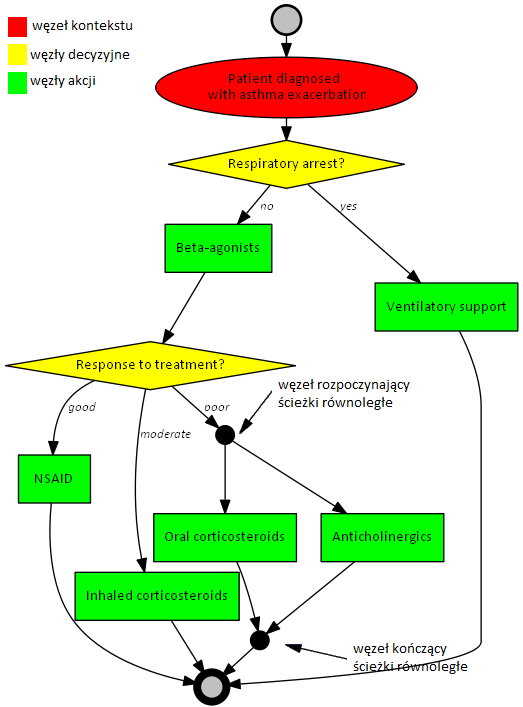
\includegraphics[width=0.7\textwidth]{img/asthma_sciezki_rownolegle.png}
\caption{Przykład ścieżek równoległych}
\label{fig:sciezki_rownolegle}
\end{figure}

% SW: czy elementami terapii są również węzły początkowy i końcowy, kontekstowy oraz węzły równoległe? Z poniższego opisu wynika, że nie. Natomiast przykład na końcu rozdziału mówi, że tak. Należy to uspójnić.
W dalszych opisach wykorzystano pojęcia \textit{terapia} oraz \textit{element terapii}. \textit{Terapia} jest to pojedyncza ścieżka w grafie. Element terapii natomiast to identyfikator węzła w przypadku węzłów akcji, natomiast dla węzłów decyzji elementem terapii są identyfikator węzła i etykieta wybranej krawędzi oddzielone znakiem zapytania. 

\section{Wykorzystywane dane}


Dane wykorzystywane oraz generowane przez program znajdują się w następujących katalogach:
\begin{itemize}
\item{\texttt{Algorytmy} – katalog zawiera pliki o rozszerzeniu DOT opisujące grafy reprezentujące dostępne wytyczne kliniczne,}
\item{\texttt{Konflikty} – katalog zawiera opisy konfliktów, jakie mogą wystąpić między wytycznymi oraz definicje zmiany, które należy wprowadzić w przypadku wystąpienia tych konfliktów,}
\item{\texttt{Grafy} – katalog zawiera zmodyfikowane grafy chorób przedstawiające aktualnie przebytą ścieżkę oraz grafy wynikowe prezentujące rozwiązania. Grafy są w dwóch formatach – tekstowym w formacie DOT oraz graficznym w formacie PNG. Podczas kończenia pracy programu zawartość tego katalogu jest kasowana}
\end{itemize}

\section{Główne klasy}
Program zaimplementowano w języku Java. Poniżej przedstawiono listę głównych klas wykorzystywanych w programie (i pojawiających się w dalszych opisach):
\begin{itemize}
\item{\texttt{AddToTherapy} - dodawanie identyfikatorów węzłów do listy opisującej konkretną terapię,}
\item{\texttt{ChocoClass} - rozwiązanie problemu CLP za pomocą solwera Choco,}
\item{\texttt{Color} - kolorowanie wierzchołków i krawędzi grafów,}
\item{\texttt{CreateTherapies} - generowanie terapii,}
\item{\texttt{ExecuteInteractions} - wprowadzanie zmian w terapiach w przypadku wykrycia konfliktów, }
\item{\texttt{GoForward} - przechodzenie do kolejnego węzła decyzyjnego, }
\item{\texttt{GraphFunctions} - przydatne metody związane z grafami, np. znalezienie węzłów docelowych określonego węzła ,}
\item{\texttt{ImageGraph} - wyświetlanie grafów, }
% SW: napisałbym raczej, że ta klasa kontroluje przejście miedzy poszczególnymi krokami działania programu
\item{\texttt{MainClass} - obsługa zdarzenia kliknięcia przycisku Dalej ,}
\item{\texttt{RadioButtonList} - tworzenie i obsługa zdarzeń list pól wyboru służących do udzielania odpowiedzi na pytania,}
\item{\texttt{Results} - wyświetlanie wyników,}
\item{\texttt{Window} - główne okno programu.}
\end{itemize}

\section{Główne kroki działania}
\label{sec:kroki}

\subsection{Wybór chorób}
Celem tego kroku jest wybór tych wytycznych, które będą brane pod uwagę przy ustalaniu terapii. W katalogu \texttt{Algorytmy} program szuka plików posiadających rozszerzenie DOT. Dla każdego takiego pliku tworzone jest pole wyboru. Pole wyboru posiada etykietę równą nazwie choroby. Utworzone pole wyboru jest następnie dodawane do globalnej listy 
pól wyboru \texttt{Window.checkBoxGroup} oraz do panelu 
znajdującego się w lewym górnym rogu okna programu (rys. \ref{fig:wybor_chorob}). 
\begin{figure}[H]
\centering
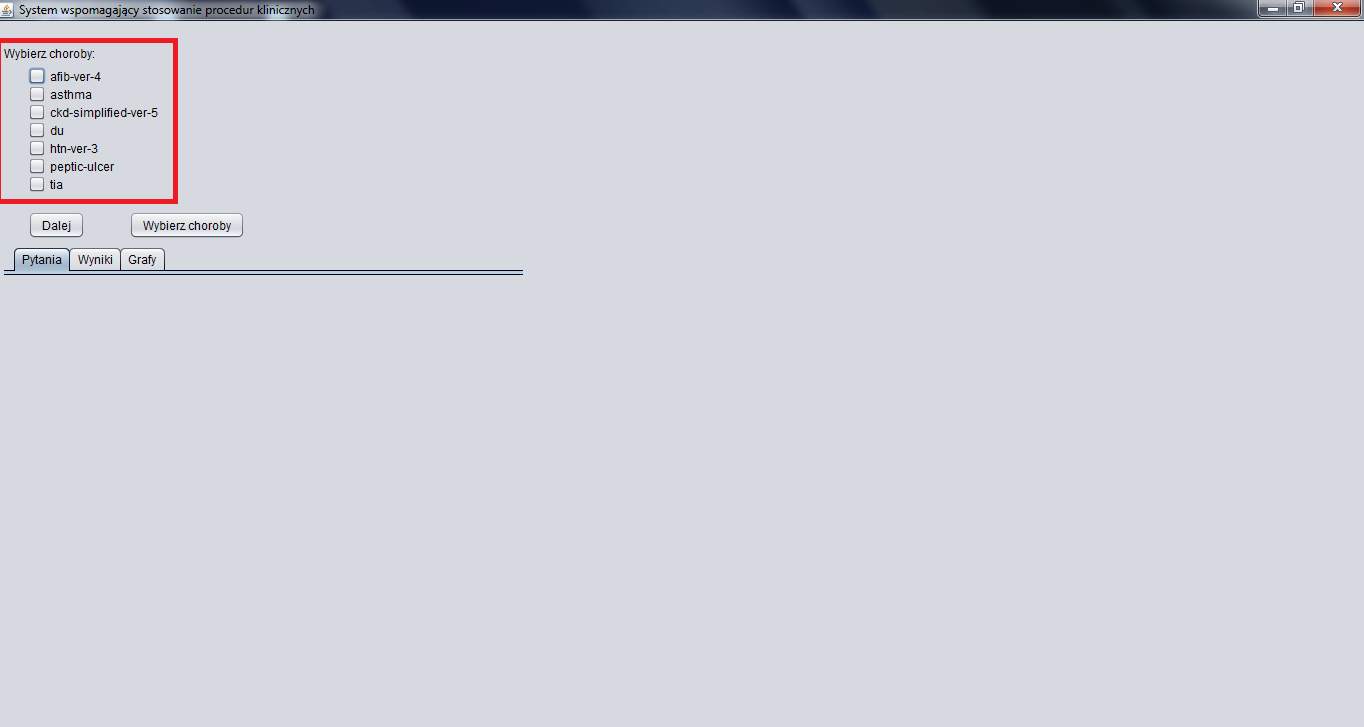
\includegraphics[width=\textwidth]{img/wybor_chorob.png}
\caption{Panel wyboru chorób}
\label{fig:wybor_chorob}
\end{figure}
Po wybraniu chorób, tzn. po kliknięciu w odpowiednie pola wyboru i kliknięciu przycisku „Dalej”, nazwy wybranych chorób są dodawane do listy \texttt{Window.selectedDiseases} i program przechodzi do fazy wyświetlania grafów oraz udzielania odpowiedzi na pytania. 

\subsection{Wyświetlanie grafów oraz udzielanie odpowiedzi na pytania}
Ten krok pozwala na utworzenie graficznej reprezentacji wytycznych oraz wybór ścieżki w grafie (terapii) zgodnej z dostępnymi danymi pacjenta. Po wybraniu chorób i kliknięciu przycisku „Dalej” program dla każdej choroby odczytuje za pomocą metody \texttt{GraphFunctions.getGraph} grafy z plików w formacie DOT. Następnie program pobiera korzenie każdego z grafów za pomocą metody \texttt{GraphFunctions.get\-StartNode}, a potem wywołuje metodę \texttt{GoForward.goForward}, która przemieszcza się po grafie (startując w jego korzeniu) do momentu, gdy napotka pierwszy węzeł decyzji. 

Metoda \texttt{goForward} dodaje aktualny węzeł do listy elementów terapii. Następnie wykonuje pętlę \texttt{while}, której warunek kontynuacji obejmuje trzy przypadki. Pierwszy warunek sprawdza, czy węzeł posiada jedną krawędź wyjściową. Drugi warunek sprawdza, czy węzeł rozpoczyna ścieżki równoległe, a trzeci czy węzeł kończy ścieżki równoległe. 

Wewnątrz pętli wykonywane są następujące akcje. Po pierwsze wykonywana jest kolejna, wewnętrzna pętla \texttt{while} (jej warunek jest taki sam, jak pierwszy z warunków w pętli zewnętrznej), aby dodać do listy elementów terapii wszystkie węzły, które mają tylko jedną krawędź wyjściową, czyli droga w grafie, po której należy się poruszać jest jednoznacznie określona. Po wykonaniu tej pętli \texttt{goForward} zatrzymuje się na węźle, który jest liściem (nie posiada żadnej krawędzi wyjściowej), albo ma więcej niż jedną krawędź wyjściową.

Następnie następuje sprawdzenie, czy aktualny węzeł rozpoczyna ścieżki równoległe (jest to też drugi warunek w pętli zewnętrznej). Jeśli warunek ten jest spełniony, wywoływana jest metoda \texttt{parallel\-Path}. Metoda ta jest wywoływana również w dla trzeciego przypadku, czyli gdy uzyskany węzeł kończy ścieżki równoległe, a program nie przeszedł jeszcze przez wszystkie te ścieżki. Metoda \texttt{GoForwared.parallel\-Path} jest w postaci pętli \texttt{while}, która działa dopóki program nie przejdzie przez wszystkie ścieżki równoległe związane z węzłem rozpoczynającym ścieżki równoległe i uzyskany węzeł 
% SW: tutaj dodałem informcje o liściu -- domyślam się, że jest to również warunek zakończenia
nie jest węzłem decyzyjnym lub liściem. Wszystkie przebyte po drodze węzły dodawane są do listy elementów terapii .  

Po wywołaniu metody \texttt{goForward} program wywołuje metodę \texttt{Color.color}, która zaznacza przebytą ścieżkę w grafie kolorując oraz pogrubiając kontury przebytych węzłów oraz przebyte krawędzie.
 
Po wywołaniu metody \texttt{color} wywołana zostaje metoda \texttt{ImageGraph.newImageGraph}, której zadaniem jest wygenerowanie i wyświetlenie nowego obrazu grafu. Na początku metoda zapisuje do pliku wynik metody \texttt{toString} wywołanej dla grafu. Następnie wywoływana jest metoda \texttt{ImageGraph.getImageGraphPath}, która uruchamia zewnętrzny program \texttt{dot} i tworzy z zapisanego wcześniej pliku tekstowego graf w postaci obrazu w formacie PNG. W kolejnym kroku metoda \texttt{ImageGraph.newImageGraph} tworzy obiekt klasy \texttt{BufferedImage} z wygenerowanym w poprzednim kroku obrazem. Później metoda dokonuje skalowania obrazu tak, aby mógł on się zmieścić w oknie (a dokładnie w przeznaczonym dla niego polu). 

Jeśli szerokość lub wysokość obrazu przekracza ustalony próg, obraz zmniejszany jest do 2/3 wielkości tak, aby był on czytelny (w tym przypadku do pola z obrazem dodawane są suwaki). Ponadto, jeżeli szerokość i wysokość obrazu jest mniejsza od wielkości pola, to na etykiecie umieszczany jest obraz bez skalowania (tzn. w skali 1:1).
 
Ostatnim krokiem jest wywołanie metody \texttt{RadioButtonList.createRadioButtonList}. Metoda ta dla każdego elementu terapii, który posiada znak zapytania tworzy panel. Elementy terapii zwierające znak zapytania odpowiadają krokom decyzyjnym. Pierwszym elementem panelu jest etykieta węzła. Pozostałe elementy stanowią pola wyboru z etykietami, których wartości są równe etykietom krawędzi wychodzących z węzła decyzyjnego. Do tych pól wyboru dodawany jest jeszcze jedno z etykietą „brak wartości”, przydatne w sytuacji, gdy dane nie są znane. Na końcu tworzony jest jeszcze jeden panel, tym razem dla pytania, na które jeszcze nie została udzielona odpowiedź -- dla niego zaznaczone jest pole wyboru z etykietą „brak wartości”. Przy pierwszym wyświetleniu grafu tworzony jest tylko ten panel. Ponadto, do każdego pola wyboru podczepiana jest metoda \texttt{RadioButtonList.updateRadioButtonList} obsługująca zdarzenia związane ze zmianą wartości pola.

Po wywołaniu metoda \texttt{updateRadioButtonList} na początku szuka elementu w liście elementów terapii, którego dotyczy wybrane pytanie (i związane z nim pole wyboru). Jeśli zaznaczone pole wyboru ma etykietę „brak wartości”, usuwane są wszystkie elementy terapii od elementu, którego dotyczy wybrane pytanie, do ostatniego elementu listy pytań. Innymi słowy następuje cofnięcie się w grafie, co oznacza, że pytania i odpowiedzi znajdujące się "poniżej" wybranej lokalizacji są odrzucane.

Jeśli natomiast zaznaczone pole wyboru nie posiada etykiety równej „brak wartości” i nie istnieje element na liście elementów terapii (użytkownik odpowiada na to pytanie po raz pierwszy), który jest związany z pytaniem, to do tej listy dodawany jest element o wartości równej \texttt{question?answer}, gdzie \texttt{answer} jest etykietą krawędzi, z którą związane jest zaznaczone pole wyboru.  Jeśli natomiast istnieje element związany z pytaniem (użytkownik modyfikuje zmienia wcześniej udzieloną odpowiedź), to w liście elementów terapii podmieniany jest element, który jest związany z pytaniem na wartość \texttt{question?answer}, a następnie usuwane są wszystkie elementy listy terapii, które się znajdują za podmienionym elementem (analogicznie jak w przypadku wyboru "braku wartości"). 

% SW: a co się dzieje, jeśli wybrano "brak wartości"? Domyślam się, że goForward nie jest wywoływane, natomiast wciąż poprawiane jest kolorowanie grafu. Jeśli tak, warto to jawnie napisać.
Następnie aktualnym węzłem staje się węzeł, do którego dochodzi krawędź związana z wybraną odpowiedzią (tzn. krawędź o etykiecie \texttt{answer} wychodzącej z węzła o identyfikatorze \texttt{question}). Węzeł ten jest punktem startowym dla kolejnego wywołania metody \texttt{goForward}. Potem metoda \texttt{updateRadioButtonList} koloruje graf na nowo na podstawie zaktualizowanej listy elementów terapii. Tworzony jest także nowy obraz grafu za pomocą metody \texttt{newImageGraph}. Na końcu tworzona jest nowa lista pytań i odpowiedzi za pomocą metody \texttt{createRadioButtonList}. 

Zaktualizowane grafy prezentowane są po prawej stronie ekranu na osobnych zakładkach. Każda zakładka dotyczy wytycznych związanych z jedną z wybranych chorób. Z lewej strony ekranu pojawiają się natomiast zakładki z listami pytań i pól wyboru pozwalającymi na uzupełnienie danych pacjenta. W tym przypadku również jedna zakładka dotyczy jednej choroby. Przykładowy ekran z grafami i polami wyboru przedstawiono na rys. \ref{fig:wyswietlanie_grafow}.
\begin{figure}[H]
\centering
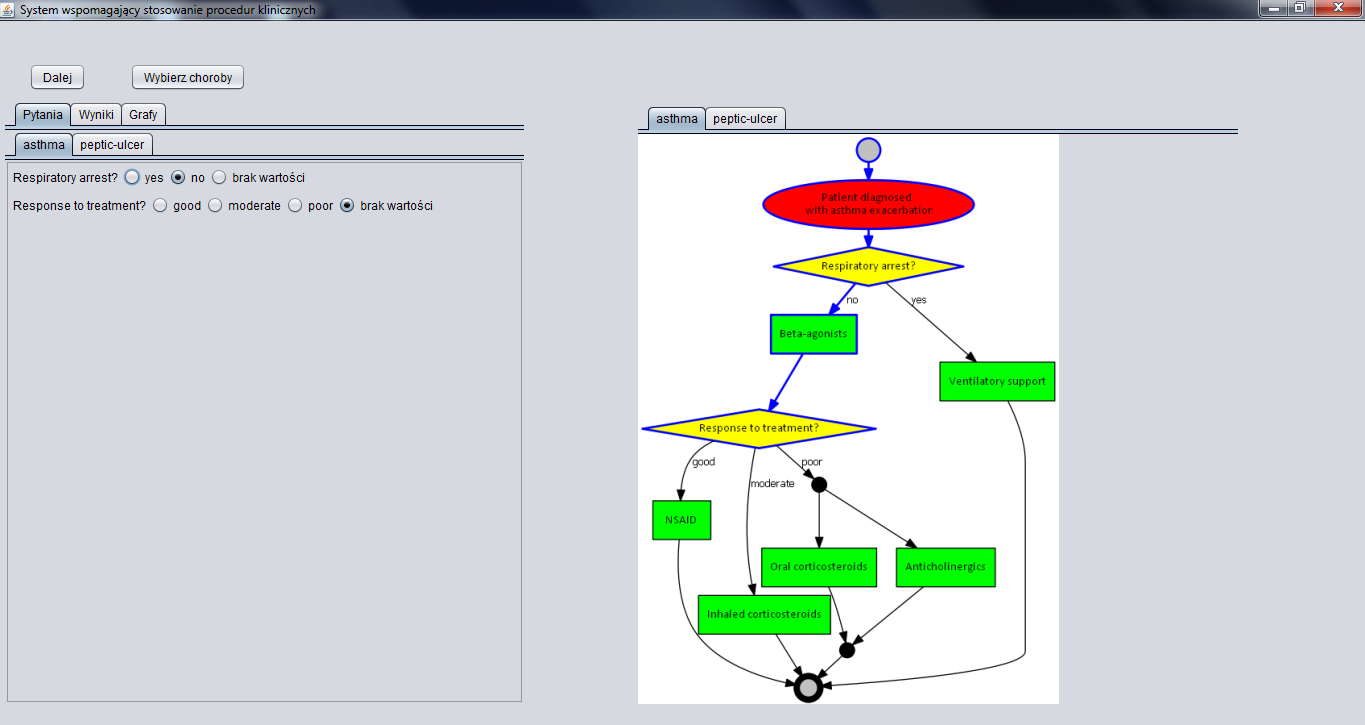
\includegraphics[width=\textwidth]{img/wyswietlanie_grafow.png}
\caption{Wyświetlanie grafów}
\label{fig:wyswietlanie_grafow}
\end{figure}

\subsection{Wyszukiwanie konfliktów}
Celem tego kroku jest znalezienie konfliktów pojawiających się między wytycznymi. Na początku program szuka w katalogu \texttt{Konflikty} plików opisujących konflikty i sposoby ich rozwiązania, które można zastosować do aktualnego zestawu wytycznych. Nazwa każdego pliku opisującego konflikty składa się z listy nazw chorób oddzielonych przecinkami (konflikty pojawiają się między wytycznymi dla tych chorób). Jeśli jakakolwiek choroba z tej listy została wybrana podczas działania programu chorobach, plik zostaje użyty. 

Plik z konfliktami zawiera jeden lub więcej wpisów (każdy poświęcony jednemu konfliktowi), a wpis (umieszczony w jednej linii) składa się z dwóch części. Pierwsza część zawiera elementy, których jednoczesne wystąpienie powoduje konflikt. Elementy te są oddzielone spacjami. Druga część zawiera zmiany, jakie należy wprowadzić w przypadku zaistnienia konfliktu. Zmiany te są oddzielone od siebie przecinkami. 
% SW: Wszystkie te listy to zmienne lokalne w metodzie ChocoClass.solve -- musiałby Pan wyjaśnić, że jest to metoda, w której rozpoczyna się poszukiwania konfliktów. Poza tym informacja o dodawaniu elementów do listy conflictsList oraz interactionsList jest przedwczesna i nieco myląca -- sugeruje proste (bezwarunkowe) dodawanie elementów do listy, podczas gdy z dalszego opisu wynika, że jest to bardziej złożone. Usunąłbym to zdanie i skupił się od razu na dodatkowych pytaniach.
Jeśli plik zostaje użyty, do listy \texttt{conflictsList} dodawane są konflikty, a do listy \texttt{interactionsList} zmiany. Ponadto, do listy \texttt{additionalQuestions} dodawane są te elementy opisujące konflikt, które oznaczają dodatkowe pytania (tzn. odwołują się do danych, które jawnie nie występują w wytycznych) -- nazwy tych elementów rozpoczynają się znakiem „\&”. Wreszcie zanegowane elementy konfliktów (rozpoczynające się od „not”) dodawane są do listy \texttt{notConflictElems}. Następnie program tworzy okienko dialogowe, które pozwala udzielić odpowiedzi na dodatkowe pytania. Pytania mogą być dwóch typów. Pierwszy typ występuje, gdy odpowiedni element konfliktu nie posiada znaku równości, mniejszości ani większości. Wtedy udzielana odpowiedź ma postać tak/nie. Drugi typ to „zmienna operator liczba”. Operator może być postaci „=”, „>”, „<”, „>=” lub „<=”. Dla tego typu elementu podawana jest wartość liczbowa w okienku dialogowym, a program sprawdza czy podana liczba spełnia warunek występujący w elemencie. 

Po udzieleniu odpowiedzi na wszystkie dodatkowe pytania program przechodzi do kolejnej części wyszukiwania konfliktów zrealizowanej w metodzie \texttt{ChocoClass.solveNextPart}. Metoda ta najpierw wywołuje metodę \texttt{ChocoClass.findSolutions}, która dla każdego możliwego konfliktu (odczytanego z pliku) wykonuje szereg operacji. Najpierw sprawdza, czy konflikt znajduje się na liście \texttt{foundConflicts}. Lista \texttt{foundConflicts} zawiera rzeczywiste konflikty, które zostały dotychczas zidentyfikowane przez program (tutaj należy zaznaczyć, że nie każdy możliwy konflikt musi zachodzić). Jeśli konflikt nie znajduje się na tej liście tworzony jest obiekt klasy \texttt{Solver}. Następnie dodawane są zmienne na podstawie wcześniej udzielonych odpowiedzi na dodatkowe pytania. Dokonuje tego metoda \texttt{ChocoClass.setAdditionalVariables}. Metoda ta sprawdza, czy pytanie jest typu tak/nie lub czy odpowiedzią na pytanie jest wartość liczbowa. W pierwszej sytuacji, jeśli odpowiedź jest równa tak, program tworzy zmienną typu \texttt{IntVar} o wartości równej jeden. Jeżeli odpowiedź jest równa nie, program tworzy zmienną \texttt{IntVar} o wartości równej zero. Jeśli odpowiedzią na pytanie jest wartość liczbowa, program tworzy zmienną \texttt{IntVar} o wartości równej podanej liczbie. 

Po wykonaniu metody \texttt{setAdditionalVariables} program wywołuje metodę \texttt{setVariables}. Metoda ta dla każdych wytycznych tworzy tablicę terapii. Dla każdej terapii (w ramach poszczególnych wytycznych) tworzona jest zmienna \texttt{IntVar} o nazwie \textit{<choroba>\_terapia<n>}, gdzie \textit{choroba} jest nazwą choroby, a \textit{n} jest indeksem terapii. Zmienna ta przyjmuje wartości zero, gdy  określona terapia nie zostaje użyta lub jeden, gdy zostaje użyta. Zmienna jest zapisywana w tablicy terapii. Następnie metoda tworzy listę \texttt{notConflictElemsTherapy}, do której dodawane są te elementy konfliktu z listy \texttt{notConflictElems}, które nie znajdują się na liście elementów konkretnej terapii, ale znajdują się w grafie związanym z terapią (innymi słowy są to te elementy, które występują w pozostałych terapiach dla danych wytycznych). 

Metoda \texttt{setVariables} tworzy też tablicę \texttt{vars}, która będzie zawierała zmienne wchodzące w skład pojedynczej terapii. Dla każdego elementu listy \texttt{notConflictElemsTherapy} w tablicy \texttt{vars} zapisywane są zmienne o nazwie \textit{not\_<X>}, gdzie X jest elementem terapii z \texttt{notConflictElemsTherapy}. Zmienna ta przyjmuje wartość 0, gdy zmienna związana z elementem terapii jest równa 1 i odwrotnie. Ponadto, dla każdego elementu terapii zapisywana jest zmienna w tablicy \texttt{vars}. Jeśli zmienna odnosi się do elementu terapii (akcji) oznaczającego podanie leku, w ramach której określono jego dawkę, tworzona jest zmienna \textit{<X>\_dosage}, gdzie \textit{X} jest elementem terapii. Następnie metoda dodaje ograniczenie mówiące, że zmienna \textit{<choroba>\_terapia<X>} przyjmuje wartość jeden, tylko wtedy, gdy suma zmiennych należących do tablicy \texttt{vars} jest równa wielkości tej tablicy (innymi słowy, gdy udało się przejść przez całą ścieżkę odpowiadającą terapii i jednocześnie nie wystąpił żaden z zanegowanych elementów konfliktu). W przeciwnym razie \textit{<choroba>\_terapia<X>} przyjmuje wartość zero. Po przejściu przez wszystkie terapie dla danych wytycznych metoda dodaje ograniczenie polegające na tym, że suma zmiennych terapii choroby ma być równa jeden, czyli dla każdej choroby ma zostać użyta tylko jedna terapia. 

Po wykonaniu metody \texttt{setVariables} program dodaje ograniczenia odpowiadające konfliktom. 
% SW: wcześniej w opisie nie ma mowy o pętli for -- należy więc wyjaśnić, że iteracyjnie sprawdzamy wszystkie możliwe konflikty odczytane z plików. W jakiej metodzie to się dzieje?
Najpierw dodawane są ograniczenia dla tych możliwych konfliktów, których udało się uniknąć (tzn. po uwzględnieniu związanych z nimi ograniczeń udało się uzyskać poprawne rozwiązanie) -- konflikty takie znajdują się na liście \texttt{avoidedConflicts}). Następnie w metodzie \texttt{ChocoClass.setConflictConstraint} dodawane jest ograniczenie dla konfliktu sprawdzanego w aktualnej iteracji pętli. Najpierw tworzy ona listę \texttt{constraintsList} przechowującą to ograniczenie. Następnie metoda iteracyjnie przetwarza elementy wchodzące w skład aktualnego konfliktu:
\begin{itemize}
\item Jeśli element konfliktu jest zanegowany (jego opis zaczyna się od "not"), do listy listy \texttt{constraintsList} dodawane jest ograniczenie \textit{not(<X> = 1)}, gdzie \textit{X} jest elementem terapii wymienionym w elemencie konfliktu. 
\item Jeśli element konfliktu zawiera jeden z operatorów "<", "<=", "=", ">", lub ">=" wówczas wywoływana jest metoda \texttt{ChocoClass.conflictWithDosage}, która sprawdza, jaki charakter ma element terapii z elementu konfliktu i dodaje odpowiednie ograniczenia do \texttt{constraintsList}. Jeśli element terapii jest związany z dodatkowym pytaniem (jego nazwa rozpoczyna się od „\&”), wówczas dodawane jest ograniczenie \textit{<X> <operator> <wartość>}, gdzie \textit{X} jest elementem terapii, a \textit{wartość} jest liczbą występującą w elemencie konfliktu. W przeciwnym razie (element terapii jest związany z akcją, w tym z podaniem leku), \texttt{constraintsList} dodawane są dwa ograniczenia. Pierwsze jest w postaci \textit{<X> = 1} (odpowiada ono wykonaniu wskazanej akcji), natomiast drugie ma formę \textit{<X>\_dosage <operator> <wartość>} i dotyczy dawki związanej z daną akcją. 
\item W pozostałych przypadkach do \texttt{constraintsList} dodawane jest ograniczenie \textit{<X> = 1}, gdzie \textit{X} to odpowiedni element terapii.
\end{itemize}

Po zakończeniu przetwarzania poszczególnych elementów konfliktu do obiektu klasy \texttt{Solver} dodawane jest ograniczenie w formie \textit{not(and(\texttt{constraintsList}))}, aby zabezpieczyć się przed wystąpieniem aktualnego konfliktu.

Następnie wywoływana jest metoda \texttt{ChocoClass.findSolutions} obiektu, które szuka rozwiązania problemu. Jeśli rozwiązanie istnieje, aktualny konflikt dodawany jest to listy do \texttt{avoidedConflicts}. Jeśli natomiast rozwiązanie nie istnieje, aktualny konflikt jest dodawany do \texttt{foundConflicts}, a do listy \texttt{interactionsList} dopisywane są zmiany powiązane z danym konfliktem. Ponadto, gdy nie ma rozwiązania program wywołuje metodę \texttt{ExecuteInteractions.execute\-Interactions}, która dokonuje zmian w wytycznych (a dokładnie w terapiach), a także program wywołuje rekurencyjnie metodę \texttt{findSolutions}, aby sprawdzić, czy wprowadzone zmiany nie spowodowały wystąpienia konfliktów, których zostały wcześniej sprawdzone, 
% SW: nie rozumiem, o co chodzi z tym "sprawdzaniem kolejnych konfliktów". Z wcześniejszego opisu wynika, że mamy metodę, która iteracyjnie je przetwarza (i nie jest to findSolutions).
oraz aby sprawdzić kolejne konflikty. 

Ostatecznie, program znajduje rozwiązania problemu z tymi ograniczeniami dla tych konfliktów, które znajdują się na liście \texttt{avoidedConflicts} (jak już wspomniano, są to konflikty, których udało się uniknąć -- dla konfliktów, które wystąpiły, wprowadzono odpowiednie zmiany do terapii). Po wygenerowaniu pierwszego rozwiązania program tworzy listę o nazwie \texttt{solutions}. Następnie w pętli, która działa dopóki istnieje kolejne rozwiązanie, program zapisuje do zmiennej \texttt{solution} nazwy zmiennych, które w rozwiązaniu posiadają wartość równą jeden. Następnie, jeśli zmienna \texttt{solution} nie znajduje się jeszcze w liście \texttt{solutions}, dodawana jest do tej listy. 

% SW: Dalsza część opisu jest zbyt szczegółowa i niezrozumiała. Rozumiem, że dla każdego rozwiazania z listy solutions identyfikujemy odpowiadające mu terapie (ścieżki w rozważancyh wytycznych), przy czym identyfikacja ta wykorzystuje zmienne pomocnicze <choroba>_terapia<n>. Co dokładnie zawiera lista therapiesDiseases -- czy jest to lista list, tzn. jej jeden element to lista możliwych terapii?

Na końcu program do listy \texttt{therapies} dodaje rozwiązania. Polega to na tym, że dla każdego elementu listy \texttt{solutions} o nazwie \texttt{elem} program tworzy listę o nazwie \texttt{therapiesSolution}. Następnie tworzy tablicę o nazwie \texttt{array} zawierającą elementy, które były w zmiennej \texttt{elem} rozdzielone przecinkami. W kolejnym kroku dla każdej choroby znajdującej się w liście \texttt{diseases} szuka elementu w tablicy \texttt{array}, którego nazwa rozpoczyna się od nazwy choroby. Następnie do listy \texttt{therapiesSolution} dodaje listę z \texttt{therapiesDiseases} o numerze równym numerowi choroby i podnumerze równym X znajdującym się w nazwie zmiennej terapii „choroba\_terapiaX”. Lista \texttt{therapiesDiseases} zawiera terapie wszystkich wybranych chorób zgodne z udzielonymi odpowiedziami na pytania znajdujące się w wytycznych. 

% SW: Tutaj powinien Pan wyjaśnić, dlaczego zmiany wprowadzane są dwukrotnie -- raz w metodzie excecuteInteractions, a raz w setGraphs. W pierwszym przypadku operujemy na ścieżkach (terapiach), a w drugim na całych grafach, co jest bardziej złożone (daje jednak lepsze możliwości wizualizacji).

\subsection{Wyświetlanie wyników}
Ostatni krok polega na wyświetleniu grafów wynikowych prezentujących rozwiązania, a także utworzeniu listy znalezionych konfliktów wraz z wprowadzanymi zmianami. Program prezentuje wyniki za pomocą metody \texttt{Results.setResults}. Na początku metoda wywołuje inną metodę o nazwie \texttt{Results.setGraphs}. 
% SW: ten opis (do końca akapitu) jest także zbyt skomplikowany -- należy tutaj wspomnieć, że modyfikujemy grafy wprowadzając niezbędne zmiany (zidentyfikowane w procesie poszukiwania rozwiązań).

Zajmuje się ona wyświetleniem rozwiązań w postaci grafów. Najpierw metoda usuwa wszystkie zakładki z rozwiązaniami z zakładki „Grafy”. W kolejnym kroku wywołuje dwie pętle, z których druga się zawiera w pierwszej. Pierwsza pętla porusza się po rozwiązaniach, druga po terapiach pojedynczego rozwiązania. Dla każdej terapii, która jest związana z określoną chorobą, tworzony jest odpowiedni graf. Następnie metoda wywołuje pętlę po grupach zmian poszczególnych konfliktów oraz po pojedynczych modyfikacjach. 

Dla każdej modyfikacji sprawdzany jest jej typ. Modyfikacje mogą być następujących typów:
\begin{itemize}
\item \textit{replace <X> with <Y>}, gdzie węzeł \textit{X} zamienia się na węzeł \textit{Y},
\item \textit{add <X> before/after <Y>}, gdzie węzeł \textit{X} jest dodawany przed lub po elemencie \textit{Y},
\item \textit{remove <X>}, węzeł \textit{X} jest usuwany,
\item \textit{increase\_dosage/decrease\_dosage <X> <DV>}, gdzie dawka leku z węzła \textit{X} jest zwiększana lub zmniejszana o wartość \textit{DV},
\item \textit{change\_dosage <X> <V>}, gdzie dawka leku z węzła \textit{X} jest ustalana na \textit{V}.  
\end{itemize}

Zmiana grafu uzależniona jest od typu modyfikacji i przeprowadzana jest w następujący sposób:
\begin{itemize}
\item Dla modyfikacji \textit{replace}, najpierw wyszukiwany jest węzeł \textit{X}. Po znalezieniu takiego węzła z pliku \texttt{Konflikty/nazwy.txt} odczytywana jest etykieta węzła \textit{Y}. Wreszcie identyfikator i etykieta znalezionego węzła są zmieniane na nowe wartości. 
\item Dla modyfikacji \textit{add}, poszukiwany jest węzeł \textit{Y}, przed lub za którym ma zostać umieszczony nowy węzeł \textit{X}. Następnie program tworzy węzeł \textit{X}, nadaje mu etykietę pobraną z pliku \texttt{nazwy.txt} i dodaje węzeł do grafu. Jeśli węzeł \textit{X} jest wstawiany po elemencie postaci \textit{pytanie?odpowiedź}, wówczas staje się on węzłem docelowym dla krawędzi z etykietą \textit{odpowiedź}, oraz wstawiana jest dodatkowa krawędź od węzła \textit{X} do poprzedniego węzła docelowego. 
% SW: Jeśli dobrze rozumiem, to jeśli wstawiamy X przed Y, to wszystkie krawędzie dochodzące do Y trafiają teraz do X oraz jest dodatkowa krawędź z X do Y. Podobnie ma się sprawa przy wstawianiu X po Y. Jeśli tak, należy dodać jeszcze odpowiednie wyjaśnienie.
W przeciwnym razie wstawiana jest krawędź z Y do X (dla \textit{add after}) lub z X do Y (dla \textit{add before}).
\item Dla modyfikacji \textit{remove} atrybuty usuwanego węzła \textit{X} modyfikowane są w taki sposób, że węzeł staje się niewidoczny na wynikowym grafie
\item Dla modyfikacji \textit{increase\_dosage}, \textit{decrease\_dosage} i \textit{change\_dosage} odpowiednio zmienia się końcową część etykiety zmienianego węzła \textit{X}, gdzie w nawiasach kwadratowych umieszczona jest zmieniona dawka leku związanego z węzłem. 

\end{itemize}

Na zakończenie metoda \texttt{setGraphs} dla każdego grafu wywołuje metodę \texttt{color} zaznaczającą przebyte węzły i krawędzie, a następnie metodę \texttt{newImageGraph}, która powoduje wygenerowanie grafu w postaci obrazkowej. 

% SW: Tak szczegółowy opis nie jest konieczny -- uprościłem go. Przydałby się jednak przykład takiej reprezentacji.
Po wywołaniu metody \texttt{setGraphs} program tworzy także tekstową reprezentację uzyskanych rozwiązań. Dla każdej z otrzymanych terapii obejmuje ona identyfikatory oraz etykiety elementów terapii (czyli odwiedzonych węzłów w grafach). Reprezentacja ta zawiera również opis napotkanych konfliktów oraz listę wprowadzonych zmian. Przy ustalaniu etykiet węzłów grafach wykorzystywane są informacje z pliku \texttt{nazwy.txt}.


\section{Przykładowe działanie programu}
W tym punkcie przedstawiono działanie programu na wybranym przykładzie klinicznym obejmującym wytyczne dla dwóch chorób: migotania przedsionków (ang. \textit{atrial fibrillation}, rys. \ref{fig:afib_przyklad}) oraz przewlekłej choroba nerek (ang. \textit{chronic kidney disease}, rys. \ref{fig:ckd_przyklad}). W przypadku węzłów odpowiadających akcjom i decyzjom podano ich etykiety oraz identyfikatory (w nawiasach okrągłych).

% SW: Sądzę, że w tych przykładach powinniśmy pokazać identyfikatory wszystkich wierzchołków, w tym początkowych, końcowych, kontekstowych (tzn. wskazujących na choroby) oraz rozpoczynających i kończących ścieżki równoległe. W opisach tekstowych do wszystkich wierzchołków odwoływałbym się poprzez ich identyfikatory -- w ten będziemy mieli bardziej zwięzły zapis.
\begin{figure}[H]
\centering
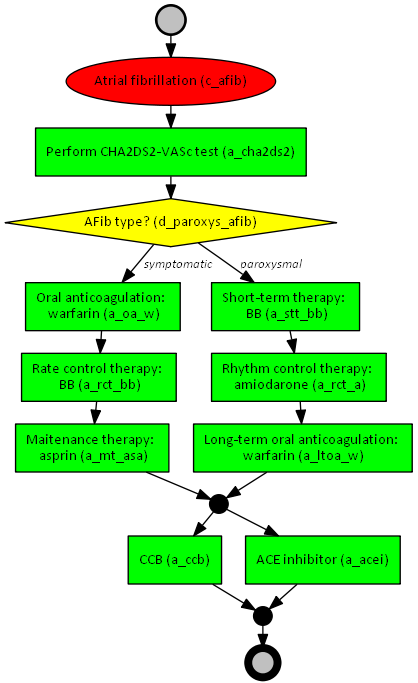
\includegraphics[scale=0.5]{img/afib-ver-4_przyklad.png}
\caption{Wytyczne dla migotania przedsionków}
\label{fig:afib_przyklad}
\end{figure}
\begin{figure}[H]
\centering
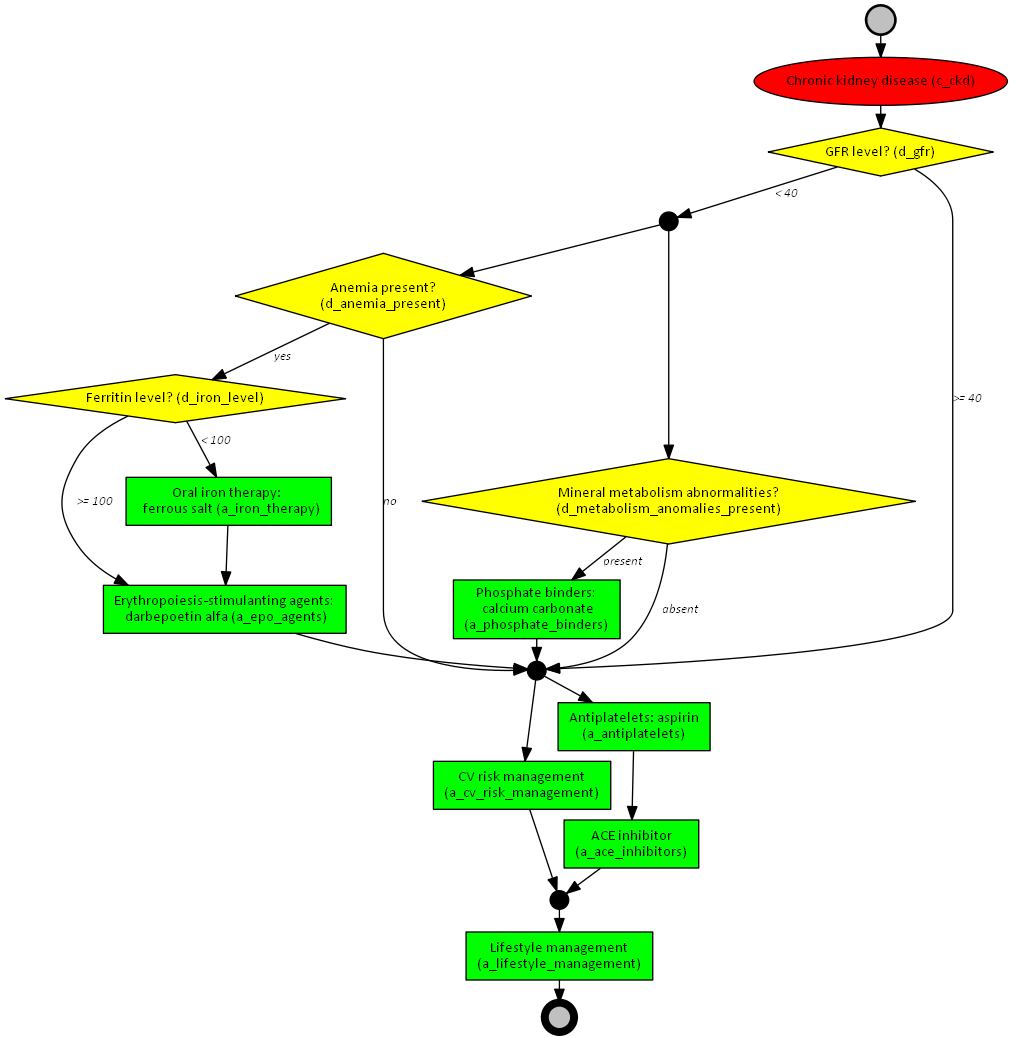
\includegraphics[scale=0.4]{img/ckd-simplified-ver-5_przyklad.png}
\caption{Wytyczne dla przewlekłej choroby nerek}
\label{fig:ckd_przyklad}
\end{figure}

W przypadku wytycznych dla migotania przedsionków (rys. \ref{fig:afib_przyklad}) program zatrzymuje się na pierwszym węźle decyzyjnym \textit{AFib type?}, zapisując wcześniej do listy elementów terapii węzeł startowy, węzeł kontekstowy określający chorobę oraz węzeł \textit{Perform CHA2DS2-VASc test}. Po wskazaniu przez użytkownika odpowiedzi \textit{paroxysmal} program dodaje do listy \textit{d\_paroxys\_afib?paroxysmal}, a następnie trzy węzły: \textit{Short-term therapy: BB}, \textit{Rhythm control therapy: amiodarone} i \textit{Long-term oral anticoagulation: warfarin}. Następnie program dodaje węzeł rozpoczynający ścieżki równoległe, następnie dwa węzły znajdujące się na ścieżkach równoległych (najpierw węzeł \textit{CCB}, następnie węzeł \textit{ACE inhibitor}), a później węzeł kończący ścieżki równoległe. Ostatecznie program dodaje węzeł końcowy grafu. 

W wytycznych dla choroby nerek (rys. \ref{fig:ckd_przyklad}) program zatrzymuje się na węźle decyzyjnym \textit{GFR level?}, dodając po drodze do listy elementów terapii węzeł startowy oraz węzeł choroby. Po udzieleniu odpowiedzi \textit{<40} program dodaje do listy \textit{d\_gfr?<40}, a następnie trafia na węzeł rozpoczynający ścieżki równoległe, który również jest dodawany do listy. W kolejnym kroku program zatrzymuje się na  decyzji znajdującej się na lewej ścieżce równoległej: \textit{Anemia present?}. Po uzyskaniu odpowiedzi \textit{no} program dodaje do listy element \textit{d\_anemia\_present?no}, a następnie wraca do prawej ścieżki równoległej i zatrzymuje się na decyzji \textit{Mineral metabolism abnormalities?}. Po uzyskaniu odpowiedzi \textit{absent} program dodaje do listy \textit{d\_metabolism\_anomalies\_present?absent}. Następnie program umieszcza na liście węzeł kończący ścieżki równoległe, który jednocześnie rozpoczyna kolejne ścieżki równoległe. W kolejnym kroku program dodaje element znajdujący się na lewej ścieżce równoległej, czyli \textit{CV risk management}, a następnie elementy znajdujące się na prawej ścieżce równoległej, czyli \textit{Antiplatelets: aspirin} oraz \textit{ACE inhibitor}. Ostatecznie dodawany jest węzeł kończący ścieżki równoległe, węzeł \textit{Lifestyle management} oraz węzeł końcowy grafu.

Po określeniu terapii program przechodzi do fazy wyszukiwania konfliktów. 
% SW: Ten plik zawiera również konflikty dla nadciśnienia -- warto o tym wspomnieć, aby wyjaśnić pojawianie się c_htn
Najpierw program odczytuje plik z konfliktami dotyczącymi migotania przedsionków oraz przewlekłej choroby nerek. Plik ten ma następującą zawartość:
\begin{verbatim}
c_htn c_ckd:remove a_step1_acei,remove a_step1_ccb
c_afib c_ckd c_htn:remove a_step3_diuretric
c_afib c_ckd:replace a_antiplatelets with warfarin,replace a_rct_a with BB
c_afib c_ckd &CHA2DS2-VASc>2:replace a_mt_asa with warfarin2
c_afib c_ckd &CHA2DS2-VASc<=1:replace a_oa_w with aspirin1,
replace a_ltoa_w with aspirin2
\end{verbatim}
Następnie program prosi o uzupełnienie danych pacjenta i podane wartości zmiennej \textit{CHA2\-DS2-VASc}. Użytkownik uzupełnia dane -- niech wartość tej zmiennej będzie równa 5, a program zaczyna wyszukiwać konflikty. Ostatecznie program znajduje dwa konflikty: (\textit{c\_afib c\_ckd} -- współwystąpienie obu chorób) oraz (\textit{c\_afib c\_ckd \&CHA2DS2-VASc>2} -- podwyższona wartość CHA2DS2-VASc w połączeniu z migotaniem przedsionków). Pierwsze dwa konflikty nie wystąpiły, ponieważ pacjent nie choruje na nadciśnienie (\textit{c\_htn}), więc odpowiednie wytyczne nie są rozważane. Ostatni konflikt nie wystąpił natomiast dlatego, że zmienna CHA2DS2-VASc przyjmuje wartość większą od 1.

W kolejnym kroku program tworzy zmodyfikowane grafy wynikowe, które zawierają zmiany wprowadzone w celu uniknięcia konfliktów. Graf dla migotania przedsionków został przedstawiony na rys. \ref{fig:afib_rozw}, natomiast graf dla przewlekłej choroby nerek jest na rys. \ref{fig:ckd_rozw}. W grafie dla migotania przedsionków węzeł \textit{Maintenance therapy: aspirin} został zmieniony na \textit{Maintenance therapy: Warfarin} oraz węzeł \textit{Rhytm control therapy: amiodarone} na węzeł \textit{BB}. Natomiast W grafie dla przewlekłej choroby nerek węzeł \textit{Antiplatelets: aspirin} został zmieniony na \textit{Warfarin}.

\begin{figure}[H]
\centering
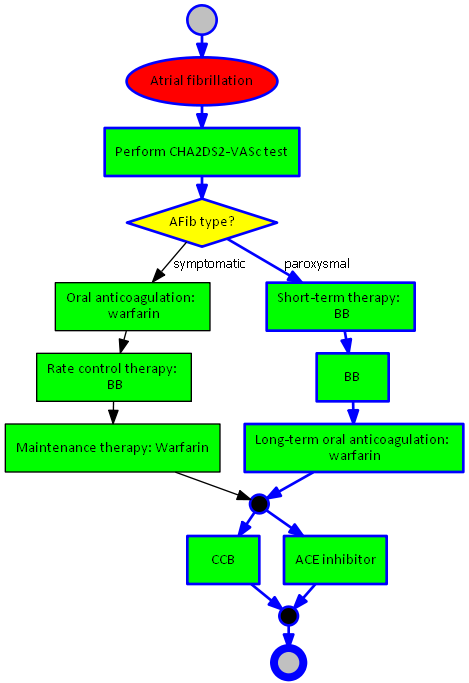
\includegraphics[scale=0.5]{img/rozwiazanie1afib-ver-4_przyklad.png}
\caption{Wytyczne dla migotania przedsionków}
\label{fig:afib_rozw}
\end{figure}
\begin{figure}[H]
\centering
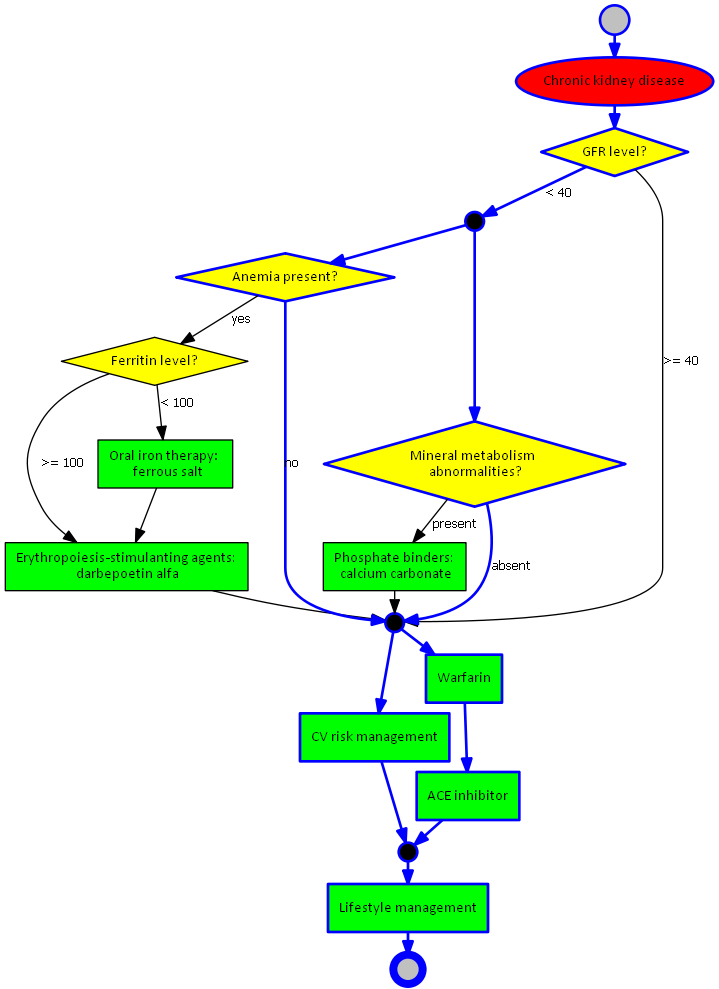
\includegraphics[scale=0.4]{img/rozwiazanie1ckd-simplified-ver-5_przyklad.png}
\caption{Wytyczne dla przewlekłej choroby nerek}
\label{fig:ckd_rozw}
\end{figure}

\chapter{Działanie systemu}
W tym rozdziale zaprezentowane zostało działanie stworzonego systemu z wykorzystaniem wybranych przykładów wytycznych klinicznych (wszystkie wytyczne zostały skonsultowane z lekarzami, przy czym część została uproszczona na potrzeby wcześniejszych publikacji, np. \citep{SzWilk,SzWilk2}). Dla każdego przykładu przedstawione zostały grafy reprezentujące zastosowane wytyczne. Na grafach tych zaznaczono ścieżki, które zostały wybrane podczas etapu zbierania danych pacjenta i udzielania odpowiedzi na pytania związane z węzłami decyzyjnymi. Odpowiedzi na pytania są także przedstawione w formie tekstowej. Następnie, dla każdego przykładu przedstawiono listę możliwych konfliktów oraz zmiany, jakie należy wprowadzić w przypadku ich wystąpienia (do opisu zmian wykorzystano składnię wprowadzoną w rozdziale \ref{sect:revisions}. W celu zachowania większej zwięzłości prezentacji w opisach konfliktów i wymaganych zmian zastosowano identyfikatory węzłów -- są one przedstawione na grafach (w nawiasach po etykietach poszczególnych węzłów). Ponadto dla każdego przykładu pogrubioną czcionką zaznaczono znalezione konflikty (nie wszystkie możliwe konflikty musiały wystąpić). Na końcu każdego przykładu podane zostały grafy wynikowe. Dodane węzły w grafach wynikowych zostały oznaczone niebieską czcionką.

\section{Przykład 1 - atak astmy i wrzód trawienny}
Wytyczne dla ataku astmy (ang. \textit{asthma exacerbation}) przedstawiono na rys. \ref{fig:ag_ae}, natomiast wytyczne dla wrzodu trawiennego (ang. \textit{peptic ulcer}) przedstawiono na rys. \ref{fig:pu}.

\begin{figure}[H]
\centering
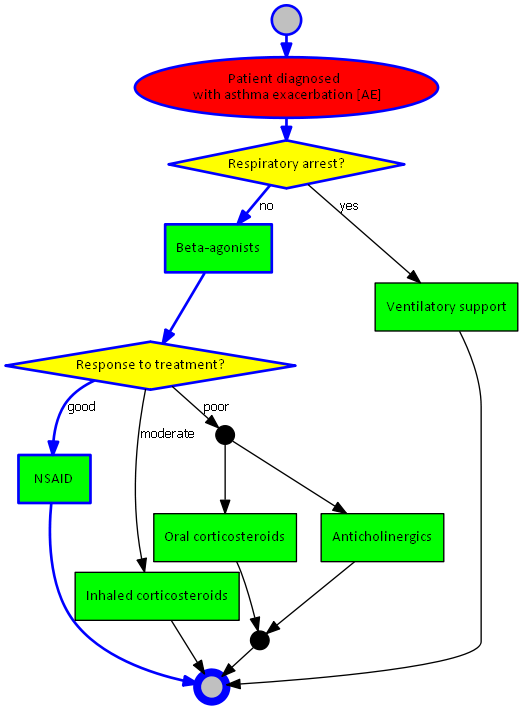
\includegraphics[scale=0.45]{img/asthma.png}
\caption{Wytyczne dla ataku astmy}
\label{fig:ag_ae}
\end{figure}

\begin{figure}[H]
\centering
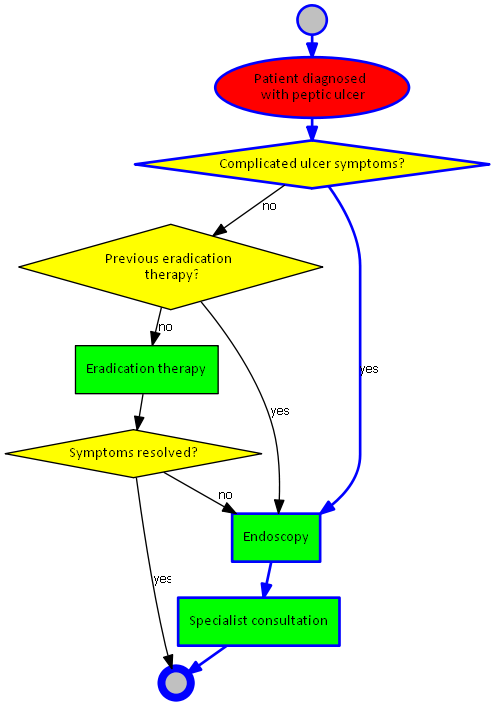
\includegraphics[scale=0.45]{img/peptic-ulcer.png}
\caption{Wytyczne dla wrzodu trawiennego}
\label{fig:pu}
\end{figure}

Dane opisujące stan pacjenta (odpowiedzi na pytania z wytycznych) są następujące:
\begin{enumerate}
\item{Atak astmy:
	\begin{itemize}
	\item{Respiratory arrest?: no (d\_arrest?no)}
	\item{Response to treatment?: good (d\_response?good)}
	\end{itemize}
}
\item{Wrzód trawienny:
	\begin{itemize}
	\item{Complicated ulcer symptoms?: yes (d\_symptoms?yes)}
	\end{itemize}
}
\end{enumerate}

Dla rozważanych wytycznych możliwe są następujące konflikty:
\begin{enumerate}
\item c\_pe a\_oral\_cortico: replace a\_oral\_cortico with a\_inh\_cortico2
\item \textbf{c\_pe a\_nsaid: add a\_ppi after a\_nsaid}
\item a\_et a\_inh\_cortico: replace a\_inh\_cortico with a\_oral\_cortico2
\end{enumerate}

% SW: W grafach wynikowych warto byłoby zaznaczyć zmodyfikowane węzły (np. innym kolorem tekstu) oraz wspomnieć o tym w opisie
Graf wynikowy dla ataku astmy przedstawiono na rys. \ref{fig:rozw_ae}, natomiast graf wynikowy dla wrzodu trawiennego jest identyczny jak ten z rys. \ref{fig:pu}.
% SW: w tym grafie należałoby zmienić opis węzła PPI -> PPI (a_ppi), aby zachować taką samą konwencję, jak w przypadku pozostałych
\begin{figure}[H]
\centering
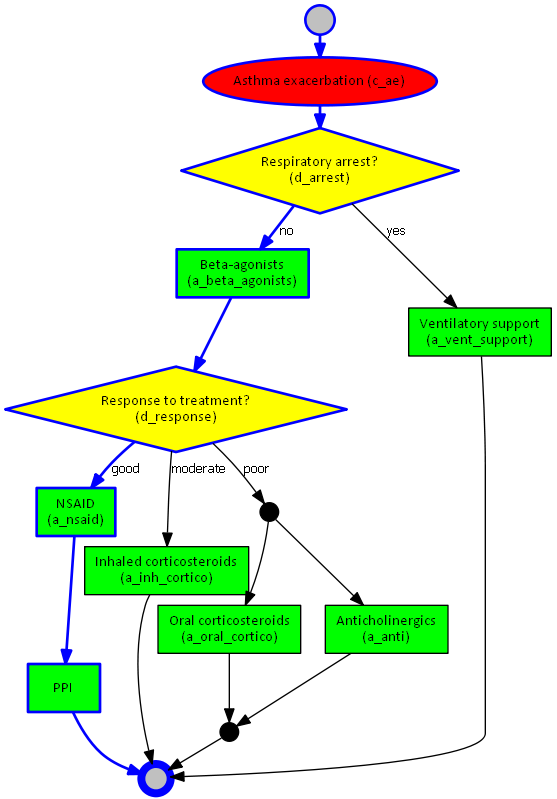
\includegraphics[scale=0.45]{img/rozwiazanie1asthma.png}
\caption{Graf wynikowy dla ataku astmy}
\label{fig:rozw_ae}
\end{figure}
\newpage
\section{Przykład 2 - migotanie przedsionków, przewlekła choroba nerek i nadciśnienie}
Wytyczne dla migotania przedsionków (ang. \textit{atrial fibrillation}) przedstawiono na rys. \ref{fig:afib}, dla dla przewlekłej choroby nerek (ang. \textit{chronic kidney disease}) na rys. \ref{fig:ckd}, a dla dla nadciśnienia (ang. \textit{hypertension}) na rys. \ref{fig:htn}.
% SW: tutaj zmiemiłbym identyfikator węzła decyzyjnego: d_paroxys_afib -> d_afib (większa spójność z innymi grafami). Podobna zmiana powinna zostać też wprowadzona do tekstu.

\begin{figure}[H]
\centering
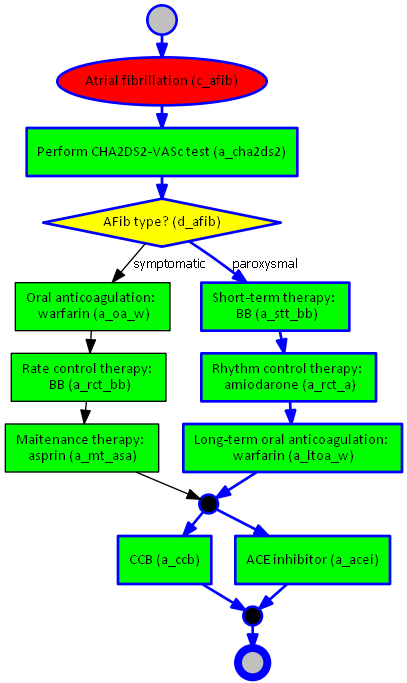
\includegraphics[scale=0.45]{img/afib-ver-4.png}
\caption{Wytyczne dla migotania przedsionków}
\label{fig:afib}
\end{figure}


\begin{figure}[H]
\centering
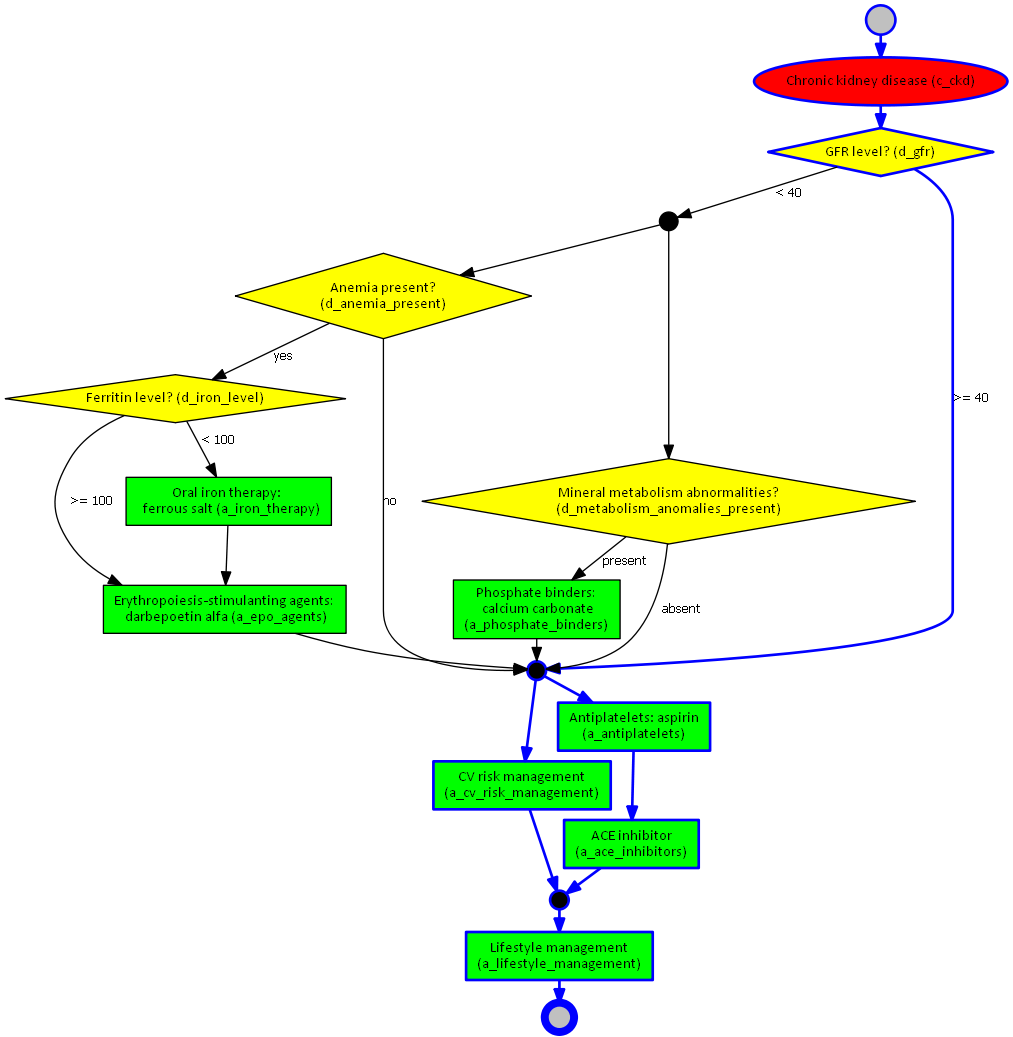
\includegraphics[scale=0.4]{img/ckd-simplified-ver-5.png}
\caption{Wytyczne dla przewlekłej choroby nerek}
\label{fig:ckd}
\end{figure}

% SW: tutaj zmieniłbym identyfikatory niektórych wierzchołków w grafie na bardziej spójne z tym, co widzieliśmy w poprzednich grafach:
% d_age_under_55 -> d_age
% d_bp_controlled_1 -> d_bp_1
% d_bp_controlled_2 -> d_bp_2
% d_bp_controlled_3 -> d_bp_3

\begin{figure}[H]
\centering
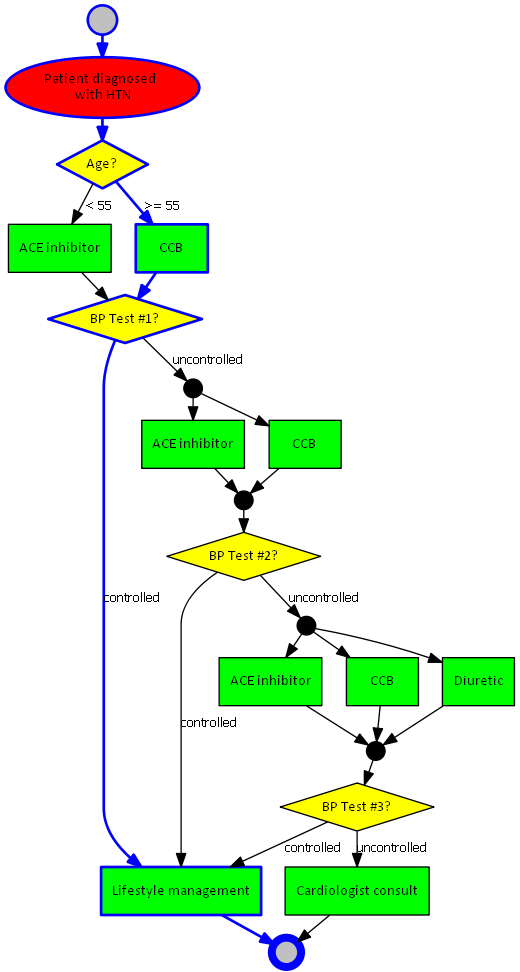
\includegraphics[scale=0.45]{img/htn-ver-3.png}
\caption{Wytyczne dla nadciśnienia}
\label{fig:htn}
\end{figure}

Dane opisujące stan pacjenta (odpowiedzi na pytania z wytycznych) są następujące:
\begin{enumerate}
\item{Migotanie przedsionków:
	\begin{itemize}
	\item{AFib type?: paroxysmal (d\_afib?paroxysmal)}
	\end{itemize}
}
\item{Przewlekła choroba nerek:
	\begin{itemize}
	\item{GFR level?: >=40 (d\_gfr?>=40)}
	\end{itemize}
}
\item{Nadciśnienie:
	\begin{itemize}
	\item{Age?: >=55 (d\_age?>=55)}
	\item{BP Test \#1?: controlled (d\_bp\_1?controlled)}
	\end{itemize}
}
\item Dodatkowe dane, które nie pojawiły się jawnie w wytycznych i które zostały uzupełnione podczas fazy poszukiwania konfliktów:
	\begin{itemize}
	\item{CHA2DS2-VASc = 5 (\&CHA2DS2-VASc?5)}
	\end{itemize}
\end{enumerate}

Dla rozważanych wytycznych możliwe są następujące konflikty:
\begin{enumerate}
\item \textbf{c\_htn c\_ckd: remove a\_step1\_acei, remove a\_step1\_ccb}
\item \textbf{c\_afib c\_ckd c\_htn: remove a\_step3\_diuretric}
\item \textbf{c\_afib c\_ckd: replace a\_antiplatelets with a\_warfarin, replace a\_rct\_a with a\_bb}
\item \textbf{c\_afib c\_ckd \&CHA2DS2-VASc>2: replace a\_mt\_asa with a\_warfarin\_2}
\item c\_afib c\_ckd \&CHA2DS2-VASc<=1: replace a\_oa\_w with a\_aspirin\_1, replace a\_ltoa\_w with a\_aspirin\_2
\end{enumerate}

Graf wynikowy dla migotania przedsionków przedstawiono na rys. \ref{fig:rozw_afib}, dla przewlekłej choroby nerek na rys. \ref{fig:rozw_ckd}, natomiast dla nadciśnienia na rys. \ref{fig:rozw_htn}.

% SW: W tym grafie powinien zmienić Pan opis węzła BB -> BB (a_bb)
\begin{figure}[H]
\centering
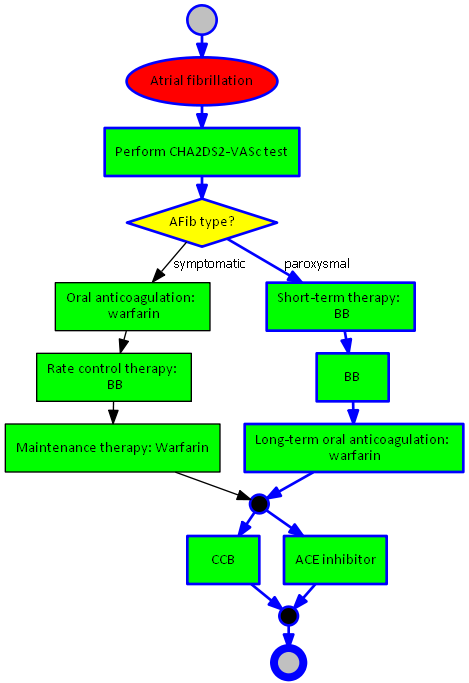
\includegraphics[scale=0.45]{img/rozwiazanie1afib-ver-4.png}
\caption{Graf wynikowy dla migotania przedsionków}
\label{fig:rozw_afib}
\end{figure}

% SW: w tym grafie zmieniamy Warfarin -> Warfarin (a_warfarin) oraz Maintenance therapy: warfarin -> Maintenance therapy: warfarin (a_warfarin_2)
\begin{figure}[H]
\centering
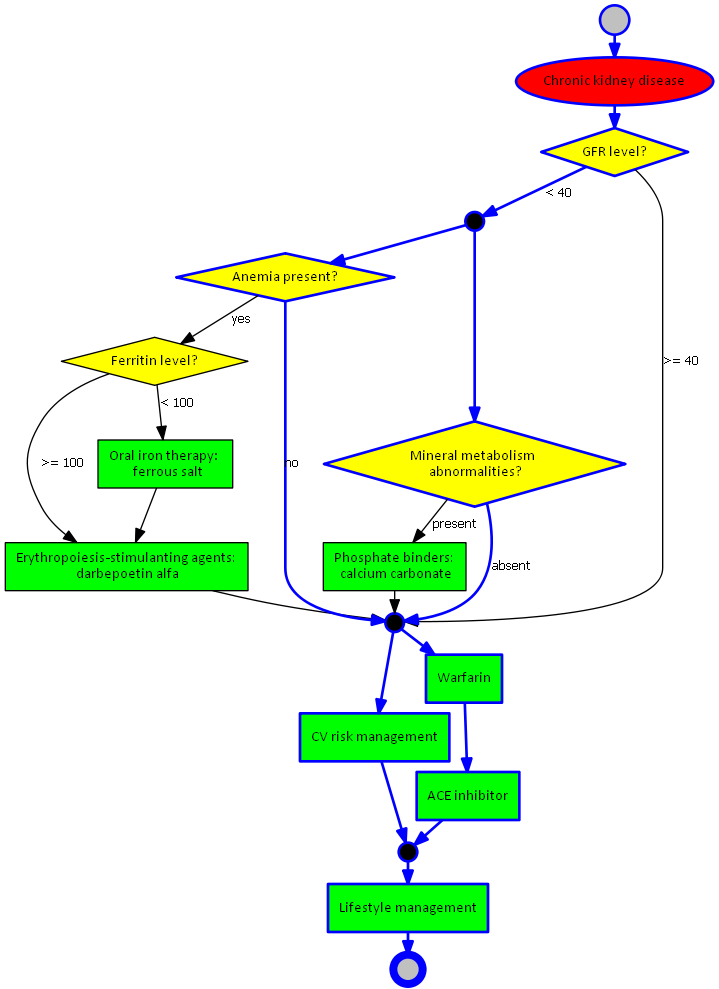
\includegraphics[scale=0.4]{img/rozwiazanie1ckd-simplified-ver-5.png}
\caption{Graf wynikowy dla przewlekłej choroby nerek}
\label{fig:rozw_ckd}
\end{figure}
\begin{figure}[H]
\centering
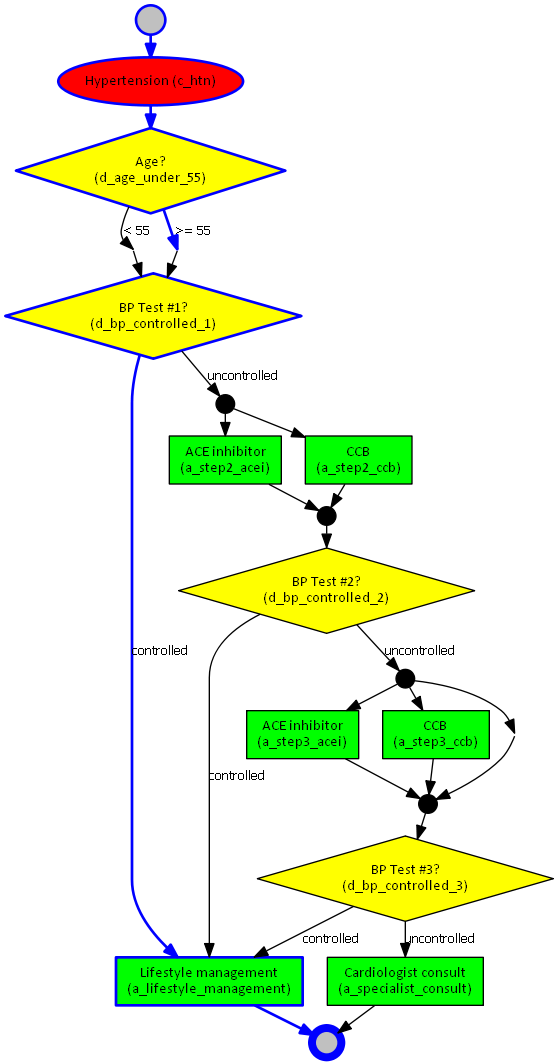
\includegraphics[scale=0.45]{img/rozwiazanie1htn-ver-3.png}
\caption{Graf wynikowy dla nadciśnienia}
\label{fig:rozw_htn}
\end{figure}


\newpage
\section{Przykład 3 - wrzód dwunastnicy i przemijający atak niedokrwienny}
Wytyczne dla wrzodu dwunastnicy (ang. \textit{duodenal ulcer}) przedstawiono na rys. \ref{fig:du}, natomiast dla przemijającego ataku niedokrwiennego (ang. \textit{transient ischemic attack}) na rys. \ref{fig:tia}.
\begin{figure}[H]
\centering
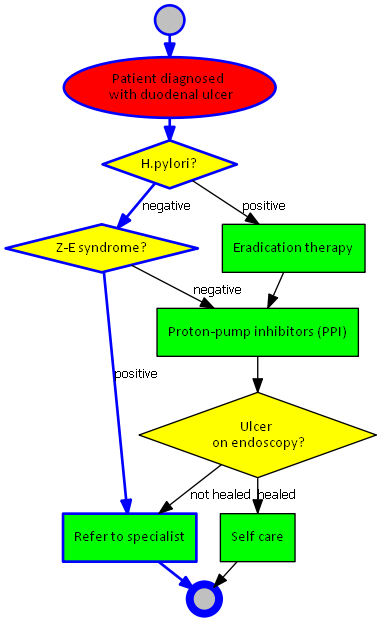
\includegraphics[scale=0.45]{img/du.png}
\caption{Wytyczne dla wrzodu dwunastnicy}
\label{fig:du}
\end{figure}


\begin{figure}[H]
\centering
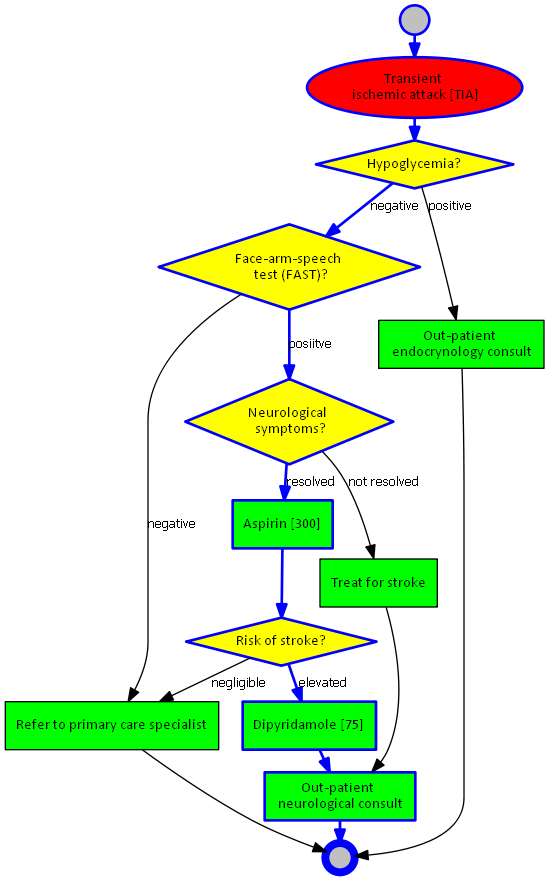
\includegraphics[scale=0.45]{img/tia.png}
\caption{Wytyczne dla przemijającego ataku niedokrwiennego}
\label{fig:tia}
\end{figure}

Dane opisujące stan pacjenta (odpowiedzi na pytania z wytycznych) są następujące:
\begin{enumerate}
\item{Wrzód dwunastnicy:
	\begin{itemize}
	\item{H.pylori?: negative (d\_hyplori?negative)}
	\item{Z-E syndrome?: positive (d\_ze\_syndrome?positive)}
	\end{itemize}
}
\item{Przemijający atak niedokrwienny:
	\begin{itemize}
	\item{Hypoglycemia?: negative (d\_hypoglycemia?negative)}
	\item{Face-arm-speech test (FAST)?: positive (d\_fast?positive)}
	\item{Neurological symptoms?: resolved (d\_neuro\_symptoms?resolved)}
	\item{Risk of stroke?: elevated (d\_stroke\_risk?elevated)}
	\end{itemize}
}
\end{enumerate}
Dla rozważanych wytycznych możliwe są następujące konflikty:
\begin{enumerate}
\item c\_du a\_aspirin not(a\_ppi) not(a\_dipyridamole): replace a\_aspirin with a\_cl
\item \textbf{c\_du a\_aspirin not(a\_ppi) a\_dipyridamole: add a\_ppi\_2 after d\_ze\_synd\-rome?positive, decrease\_dosage a\_aspirin 50}
\end{enumerate}

Graf wynikowy dla wrzodu dwunastnicy przedstawiono na rys. \ref{fig:rozw_du}, natomiast dla przemijającego ataku niedokrwiennego na rys. \ref{fig:rozw_tia}.

% SW: W tym grafie proszę zmienić Proton-pump inhibitors (PPI) -> Proton-pump inhibitors (a_ppi_2)
\begin{figure}[H]
\centering
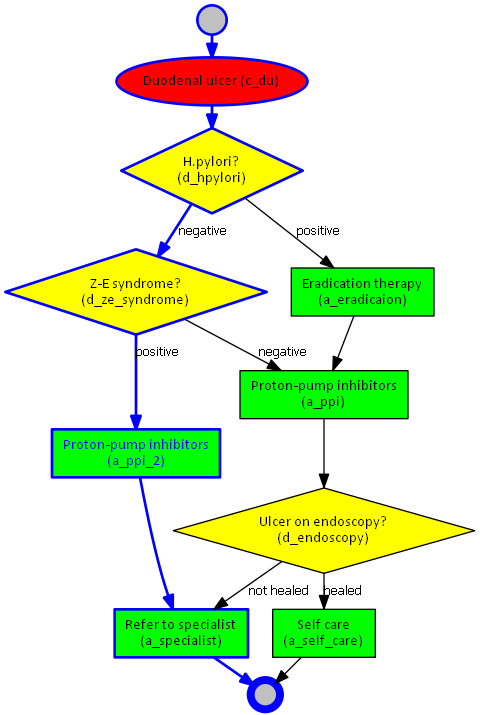
\includegraphics[scale=0.5]{img/rozwiazanie1du.png}
\caption{Graf wynikowy dla wrzodu dwunastnicy}
\label{fig:rozw_du}
\end{figure}
\begin{figure}[H]
\centering
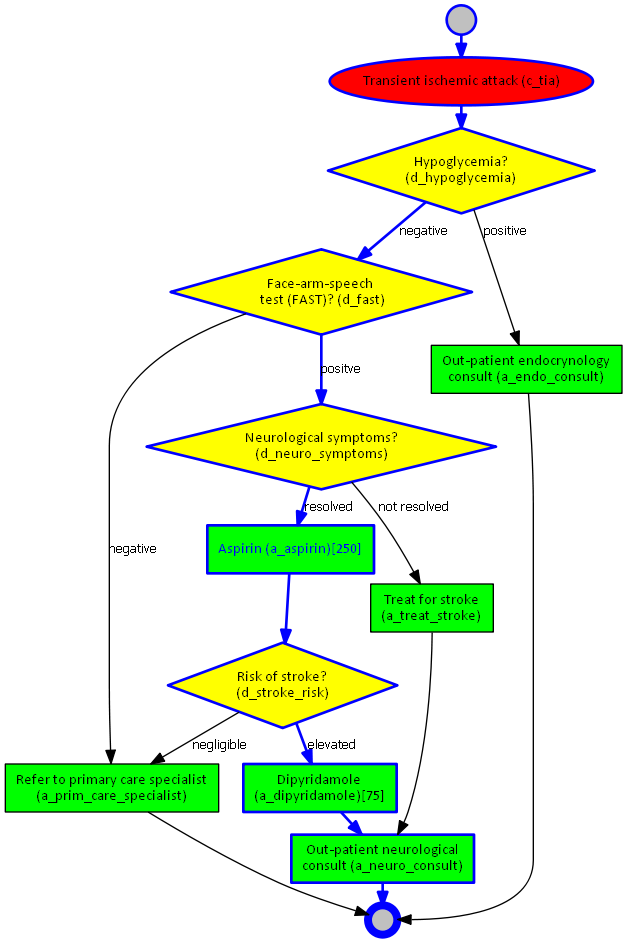
\includegraphics[scale=0.5]{img/rozwiazanie1tia.png}
\caption{Graf wynikowy dla przemijającego ataku niedokrwiennego}
\label{fig:rozw_tia}
\end{figure}


\chapter{Podsumowanie}

\section{Osiągnięte cele}
% SW: Tutaj warto jeszcze raz krótko opisać, jakie cele postawiliśmy sobie przy realizacji tej pracy (uogólnienie podejścia bazującego na CLP oraz implementacja rozszerzonego podejścia w formie interaktywnego SWDK).

Podsumowując, wszystkie zamierzenia pracy zostały zrealizowane. Wynikiem pracy jest działający program wyszukujący konflikty występujące między stosowanymi terapiami chorób i proponujący rozwiązania ewentualnych konfliktów. 

\section{Problemy przy realizacji pracy}
% SW: Czy konieczność opanowania nowej metodologii (CLP) oraz powiązanych narzędzi nie stanowiła również pewnego problemu? Jeśli tak, to warto o tym wspomnieć w tym miejscu, podkreślając, że udało się tego Panu dokonać.
Do problemów przy realizacji pracy należy zaliczyć kwestię związaną z wyborem biblioteki służącej do przetwarzania grafów. Ostatecznie wybrana została biblioteka JPGD, ponieważ jest to dość prosta biblioteka. W bardzo łatwy sposób uzyskuje się dostęp do obiektu klasy Graph i podrzędnych obiektów klas Node oraz Edge. Niestety, skorzystanie z tej biblioteki wiązało się z naprawą pewnych błędów związanych z ponownym uzyskiwaniem grafu w wersji tekstowej. Konieczna była modyfikacja funkcji toString dla klas Graph, Node oraz Edge, ponieważ generowane początkowo przez bibliotekę grafy w wersji tekstowej nie pozwalały na wygenerowanie grafu w wersji obrazkowej przez program dot.exe. Przyczyna błędu tkwiła w tym, że biblioteka nie radziła sobie z pustymi wartościami atrybutów. Ponadto, trzeba było zrezygnować z korzystania z podgrafów, ponieważ były one niewłaściwie przez bibliotekę interpretowane. 

Kolejnym problemem przy realizacji pracy była konieczność zapoznania się z bibliotekami Choco, JPGD oraz oprogramowaniem Graphviz. W przypadku bibliotek Choco i JPGD konieczne było zrozumienie ich dokumentacji. Jeśli chodzi o Graphviz, to główny problem stanowiło zapoznanie się z działaniem programów do tworzenia grafów w formie konsolowej (dot.exe) oraz okienkowej (gvedit.exe).

\section{Kierunki dalszego rozwoju}

% SW: Kierunki dlaszego rozwoju można podzielić na te związane z samym podejściem (metodą) oraz na te związane z programem (implementacją). W ramach tych pierwszych można wspomnieć o uwzględnianiu czasu w wytycznych oraz konfliktach (np. konflikty zachodzą, jeśli dwie akcje wykonywane są w tym samym oknie czasowym -- w przeciwnym razie konfliktu nie ma) oraz o uwzględnianiu kosztów podczas usuwania konfliktów (jeśli kilka sposobów usunięcia konfliktu jest możliwych, wówczas wybieramy ten "najtańszy"). Jeśli chodzi o natomiast o implementację, to tutaj można rozważyć inne metody interakcji (w tym większą "klikalność"), połączenie z zewnętrznymi systemami w celu importu danych pacjenta oraz przygotowanie wersji mobilnej.

Kierunki dalszego rozwoju dzielą się na kierunki związane z podejściem oraz związane z implementacją. Do tych pierwszych można zaliczyć uwzględnianie czasu w wytycznych i konfliktach, które polegałoby na tym, że konflikt występuje wtedy, gdy dwie akcje są wykonywane w tym samym czasie. Ponadto, do kierunków związanych z podejściem mogłoby należeć uwzględnianie kosztów w konfliktach. Wtedy metoda wybierałaby rozwiązanie konfliktu o najmniejszym koszcie. 

Jeśli chodzi o implementację, to dalszy rozwój projektu mógłby dążyć do bardziej interaktywnej odpowiedzi na pytania. Program mógłby pozwalać na klikanie na krawędzie grafu zamiast wybierać odpowiedzi za pomocą 
% SW: Termin "radiobutton" ma charakter slangowy -- lepiej mówić o "polu wyboru".
pól wyboru. Ponadto, program mógłby wspierać także inne formaty grafów, nie tylko format Graphviza o rozszerzeniu dot. Dobrymi pomysłami byłyby także integracja programu z zewnętrznymi systemami w celu pobrania danych pacjenta oraz przygotowanie wersji na aplikacje mobilne.




\backmatter
\addcontentsline{toc}{chapter}{Bibliografia}
% rodzaj bibliografii
\bibliographystyle{plain}
% plik z wpisami bibliograficznymi
\bibliography{bibliografia}

\end{spacing}
\end{document}